\chapter{Exceptions}\label{chapter:exceptions}

\section{Overview}
Many languages offer support for exceptions. You will have used exceptions in \texttt{Java} and \texttt{OCaml}.

In this chapter, we will first recap what exceptions are. Second, we will consider how to implement exceptions. Third, with a deeper understanding of how exceptions work, we will consider some subtleties regarding exceptions. Finally, in a series of optional sections, we will see exceptions as a specific example of \textit{delimited control}.

\section{Exception Semantics}
Extending a language with exceptions requires adding two constructs: 
\begin{enumerate}
    \item The ability to raise an exception
    \item The ability to handle an exception
\end{enumerate}

In this section, we will figure out, conceptually, what each of these constructs do. Once we have a precise conceptual model, we will (in an optional section) give them a formal semantics. 

\subsection{Raise}
We shall first try to extend our language with \texttt{raise}, ignoring \texttt{handle}. Once we consider \texttt{handle}, we will return and correct our semantics for \texttt{raise}.

The \texttt{raise} construct looks, abstractly, like
\[\texttt{raise}\, e\]
Where we first evaluate $e$ to some exceptional value $v$ (in a strongly typed language, exceptional values have their own type), and then raise or throw $v$.

Importantly, \textbf{ignoring \texttt{handle}}, \texttt{raise} \textit{discards} ``the rest of the computation''. That is, we have 
\[\begin{array}{rcl}
     (\texttt{raise}\, \texttt{E}(4)) + 1&\leadsto&\texttt{E}(4)  \\
     \texttt{while}\, \texttt{True} \, \texttt{do} \, \texttt{raise} \, \texttt{E}(4) & \leadsto& \texttt{E}(4)\\
     \texttt{if}\, \texttt{raise} \, \texttt{E}(4) \, \texttt{then} \, 5 \, \texttt{else} \, 7 & \leadsto&\texttt{E}(4)
\end{array} \]
The ``rest of the computation'' is specified as an evaluation context $C$. \textbf{Ignoring \texttt{handle}}, we write
\[C[\texttt{raise} \, v] \leadsto v\]
To illustrate that the context has been discarded. We consider this more thoroughly in the next, optional, sub-section.

\subsubsection{Operational Semantics of \texttt{raise} (without \texttt{handle}) \optional}
If, in \textsf{Part IB Semantics of Programming Languages}, you were asked to give an operational semantics to exceptions, you might have found it rather tricky. The reason for this is that the course shows you how to specify a \textit{local} semantics. For example, take the rules

\begin{minipage}{0.4\textwidth}
\begin{center}
    \AxiomC{}
    \UnaryInfC{$(\lambda x. e')v \leadsto [v/x]e'$ }
    \DisplayProof
\end{center}
\end{minipage}%
\begin{minipage}{0.6\textwidth}
\begin{center}
    \AxiomC{$e_1 \leadsto e_1'$}
    \UnaryInfC{$\texttt{if} \, e_1 \, \texttt{then} \, e_2 \, \texttt{else} \, e_3  \leadsto \texttt{if} \, e_1' \, \texttt{then} \, e_2 \, \texttt{else} \, e_3$ }
    \DisplayProof
\end{center}
\end{minipage}

In the rule on the left, you say, if I pattern match on my expression and find it is of the form $(\lambda x. e')v$ (one such example might be $(\lambda x. x>1)2$) then I will take the body of the function $e'$ ($x>1$), and wherever I see $x$, I will substitute $v$ ($2$).

In the rule on the right, you are saying, if I pattern match on my expression and find it is an \texttt{if} statement, then I need to evaluate the conditional to determine which branch to take. 

In using the rule on the right, you might try to solve a sub-goal, that invokes the rule on the left. For example, if you have the expression
\[\texttt{if} \, (\lambda x. x>1)2 \, \texttt{then} \, e_2 \, \texttt{else} \, e_3\]
Then you will first use the rule on the right to determine that you need to evaluate $(\lambda x. x>1)2$, which then requires the rule on the left. 

The reason why you can invoke the rule on the left like this is because the rule on the left will never have an impact on whether, or how, you use the rule on the right. For this reason, we say the semantics we have given are \textit{local}. We can hone in on any sub-expression, and solve them independently of each other. 

In contrast, consider the expression
\[\texttt{if} \, \texttt{raise} \, \texttt{E}(4)\, \texttt{then} \, e_2 \, \texttt{else} \, e_3\]
We attempt to do the same thing. We deploy the rule on the right, figure we need to try and evaluate $\texttt{raise} \, \texttt{E}(4)$, but this tells us we should throw away the rest of the \texttt{if} statement. Solving a sub-goal (evaluate \texttt{raise} $\texttt{E}(4)$) can cause us to change our original goal (evaluate the \texttt{if} expression) , and our semantics are no longer local. 

Before we deal with non-local semantics, we first make explicit this notion of goal and sub-goal. We do so by introducing evaluation contexts, $C$, which identify ``holes'' in which evaluation may take place. Examples of evaluation contexts include 

\begin{minipage}{0.33\textwidth}
    \begin{center}
        $(\lambda x. e') -$
    \end{center}
\end{minipage}%
\begin{minipage}{0.33\textwidth}
    \begin{center}
        $\texttt{if}\, - \, \texttt{then}\, e_2 \, \texttt{else} e_3$
    \end{center}
\end{minipage}%
\begin{minipage}{0.33\textwidth}
    \begin{center}
        $\texttt{if}\, (\lambda x. e') - \, \texttt{then}\, e_2 \, \texttt{else} e_3$
    \end{center}
\end{minipage}%

A non-example of an evaluation context in \textit{L2} is

\begin{center}
        $\texttt{if}\, e_1 \, \texttt{then}\, - \, \texttt{else} \, e_3$
\end{center}

Since it implies you are evaluating a branch before evaluating the conditional, which the semantics of \textit{L2} do not allow. 

Evaluation contexts allow us to say ``Evaluate this sub-expression as a sub-goal in evaluating the entire expression. Evaluating the sub-goal will never change what or how we evaluate.''. We write

\begin{center}
    \AxiomC{$e \leadsto e'$}
    \UnaryInfC{$C[e] \leadsto C[e']$ }
    \DisplayProof
\end{center}

Which means, if as a sub-goal, we find that $e$ evaluates to to $e'$, then it also evaluates to $e'$ in some context $C$. This helps us make progress in evaluating $C[e]$. Note that $C$ is unchanged, since evaluating the sub-goal does not change what or how we evaluate. 

Of course, raising an exception does change what and how we evaluate. Specifically, raising an exception ``throws away'' the rest of the computation, or the goal. Hence, \textbf{ignoring \texttt{handle}}, we write

\begin{center}
    \AxiomC{}
    \UnaryInfC{$C[\texttt{raise} \, v] \leadsto v$ }
    \DisplayProof
\end{center}

By abandoning the context in which we were evaluating \texttt{raise} $v$, we allow the evaluation of exceptions to affect what, and how we evaluate. Specifically, we allow them to \textit{throw away} our previous objectives.

\subsection{Handle}\label{section:exception-semantics:handle}
Next, we will extend our language with \texttt{handle}. The \texttt{handle} construct looks, abstractly, like
\[\texttt{try}\, e_1 \, \texttt{with} \, x \to \, e_2 \]
If an exception is raised, then \texttt{handle} \textit{catches} the raised exception and performs some operation on it. Otherwise, \texttt{handle} is not called. Concretely,
\[\begin{array}{rrccl}
     1+\texttt{try}& 2+3\, & \texttt{with} \, \texttt{E}(x) \to x+10 &\leadsto^*&6  \\
     1+\texttt{try}& 2+\texttt{raise}\, \texttt{E}(5)\, & \texttt{with} \, \texttt{E}(x) \to x+10 &\leadsto^*&16
\end{array}\]
Abstractly, given 
\[\texttt{try}\, e_1 \, \texttt{with} \, x \to \, e_2 \]
We are in one of two cases: 
\begin{enumerate}
    \item $e_1$ ($2+3$) reduces to some value $v$ ($5$), and so the entire \texttt{handle} block reduces to $v$ ($5$)
    \item $e_1$ ($2+(\texttt{raise}\, \texttt{E}(5))$) reduces to a raise statement ($\texttt{raise} \, \texttt{E}(5)$) in some context $C_2$ ($2 + -$). The handler, $e_2$ ($\lambda \texttt{E}(x). x+10$) is called on the raised value (to give $5+10 = 15$)
\end{enumerate}
In both cases, the surrounding context $C_1$ ($1+-$) is unaffected (hence evaluation results in 6 and 16, respectively). Informally, the \texttt{handle} construct \textit{contains} the effect of the \texttt{raise}.

Further, \textit{handle} \textit{handles} the raised exception value, by replacing the discarded computation with some function. In the earlier example, we replace the discarded computation $- + 1$ with the handler $- + 2$. This substitute for the discarded computation is specified by the handler body. 

We will now correct our informal semantics for \texttt{raise}. We said that $\texttt{raise} \, v$ discards \textit{all of the rest of the computation}. As we have seen, this is not true if $C$ contains a handle! The \texttt{handle} should contain the effect of \texttt{raise}, protecting anything that comes after it. Hence, \texttt{raise} should discard the rest of the computation up to (and including) the \textbf{most recent} handle. The most recent handle is replaced by the handling code in its body.

\subsubsection{Operational semantics for \texttt{raise} (with \texttt{handle}) \optional}
We will now correct our formal semantics for \texttt{raise}. We said that $\texttt{raise}$ needs to discard the computation up to and including, the most recent handle, which is replaced by its handling body. To illustrate the protective effect of the handle, we write:

\begin{center}
    \AxiomC{}
    \UnaryInfC{$C_1[\texttt{try} \, C_2[\texttt{raise} \, v] \, \texttt{with} \, x \to e_2] \leadsto C_1[[v/x]e_2]$ }
    \DisplayProof
\end{center}

This makes clear that we only discard the context $C_2$ within the \texttt{try} block.

To make clear that the \texttt{handle} is the \textit{most recent such}, we say that $C_2$ does not contain any \texttt{handle} statements. Formally, we write

\begin{center}
    \AxiomC{$\nexists C_3, C_4, e' . \; C_2 = C_3[\texttt{handle} \, C_4 \, \texttt{with} \, y \to e']$}
    \UnaryInfC{$C_1[\texttt{try} \, C_2[\texttt{raise} \, v] \, \texttt{with} \, x \to e_2] \leadsto C_1[\texttt{try} \, \texttt{raise} \, v \, \texttt{with} \, x \to e_2]$ }
    \DisplayProof
\end{center}

\subsubsection{Operational Semantics of \texttt{handle} \optional}
Since the \texttt{handle} contains the effect of a \texttt{raise}, its semantics can be specified without reference to its surrounding context. In fact, its rules are very easy

The first rule is a congruence rule

\begin{center}
    \AxiomC{$e_1 \leadsto e_1'$}
    \UnaryInfC{$\texttt{try} \, e_1 \, \texttt{with} \, x \to e_2 \leadsto \texttt{try} \, e_1' \, \texttt{with} \, x \to e_2$ }
    \DisplayProof
\end{center}

The second rule is a reduction rule that specifies what to do if no exception is raised

\begin{center}
    \AxiomC{}
    \UnaryInfC{$\texttt{try} \, v \, \texttt{with} \, x \to e_2 \leadsto v$ }
    \DisplayProof
\end{center}

The case where an exception is raised is specified under the operational semantics for \texttt{raise}.

If you try to specify these rules within a surrounding context $C$, you'll notice that you do nothing to $C$ -- that's a sign that you can drop the context from your operational semantics.

\subsection{A note on notation}
In some papers, you might see $C[e]$ written as $\langle e, C \rangle$ or $\langle e \mid C \rangle$

You may also see $C$ being referred to as $E$ (for \textbf{E}valuation context) and $K$ (for continuation).

\subsection{Exceptions in \texttt{OCaml}}
As a concrete example of exceptions, here's the exception handling syntax for exceptions in \texttt{OCaml}

\subsubsection{Exception Types}
In \texttt{OCaml}, the type of exceptions, \texttt{exn}, is defined as some extensible type
\[\texttt{type exn} \, \texttt{=} \, \ldots\]
It is extensible so that the user can extend it with exceptions of their own
\[\texttt{type exn} \, \texttt{+=} \, \texttt{E of String} \]
This is similar to how one \textit{subclasses} the \texttt{Exception} class in \texttt{Java}.

\subsubsection{Raising and Handling Exceptions}
In \texttt{OCaml}, we raise exceptions as follows
\[\texttt{raise}(\texttt{E ""})\]
And handle them using the construct
\[\texttt{try} \,e \, \texttt{with} \, \texttt{E} \, \to e_1 \]
\texttt{OCaml} also supports the pattern matching syntax
\[\begin{array}{ll}
    \texttt{try} \,e \, \texttt{with} & \; \, \, \texttt{E}_1 \, \to e_1  \\ 
    & \mid \texttt{E}_2 \, \to e_2 \\
    & \ldots
\end{array}   \]
Which is just syntactic sugar for 
\[\begin{array}{ll}
    \texttt{try} \,e\, \texttt{with} & \texttt{match} \, v \, \texttt{with} \\
    & \mid \texttt{E}_1 \, \to e_1  \\ 
    & \mid \texttt{E}_2 \, \to e_2 \\
    & \ldots
\end{array}   \]

\section{Implementing Exceptions}
In this section, we will illustrate how to implement exceptions in \texttt{JargonVM}. We will first describe how exceptions manipulate the stack (\Cref{section:stack-manipulation}). This will help us develop a set of low-level instructions for implementing exceptions. Following this, we will illustrate a semantically equivalent, but more efficient way to manipulate the stack (\Cref{section:exception-pointers}). We will then update the specification of each low-level instruction to use this optimised technique. Finally, we will illustrate a \textit{compilation scheme}: showing how we can compile the high level \texttt{raise} and \texttt{try/with} syntax into our low-level instructions.

\subsection{Exceptions: A Stack's Perspective}\label{section:stack-manipulation}
\begin{figure}[H]
    \centering
    \scalebox{0.7}{\import{figures}{stack-searching}}
    \caption{Searching the stack for the \texttt{handle} closest to the top of the stack. All stack frames between the \texttt{handle} and the \texttt{raise} are discarded}
    \label{fig:stack-searching}
\end{figure}
$C$ is the \textit{continuation}, the ``rest of the computation''. As we showed in \Cref{chapter:cps}, this continuation corresponds to the stack. Therefore, we can look at the meaning of the operational semantics in a slightly new light:

\begin{enumerate}
    \item \texttt{handle} frames are pushed onto the stack
    \item If no exception is raised, then \texttt{handle} frames are silently popped off the stack.
    \item On a \texttt{raise}, we discard \textit{the stack} ($C_2$) up to, and including, the \texttt{handle} \textit{closest to the top of the stack} (most recent \texttt{handle}). This is illustrated in \Cref{fig:stack-searching}. We then invoke the handling code.
\end{enumerate}

\subsubsection{Handler Frames}
We should also consider the structure of a handler frame. This should contain all the information needed to handle a raised exception. When an exception is raised, we need to:
\begin{enumerate}
    \item Discard the stack frames up to, and including, the handler frame, and
    \item Transfer control to the handling code
\end{enumerate}

After discarding the relevant stack frames, the frame pointer might no longer be pointing at the activation frame at the top of the stack. In order to restore the invariant, we need to restore the frame pointer to the value it was at the point when the handler frame was pushed onto the stack (\textbf{fp}). We save \textbf{fp} onto the stack.

In order to transfer control to the handling code ($e_2$ in \texttt{try} $e_1$ \texttt{with} $x \to e_2$), we use a code pointer. After compilation, $e_2$ will be some consecutive series of instructions with an address / location. We thus also need a code pointer, \textbf{cp}, that points to the address of $e_2$ in the compiled code. The structure of the handler frame is shown in \Cref{fig:handler-frame}.

\begin{figure}[H]
    \centering
    \import{figures}{handler-frame}
    \caption{The structure of a handler frame}
    \label{fig:handler-frame}
\end{figure}

This perspective is important because it helps us outline a specification for the instructions we need to introduce:

\begin{enumerate}
    \item We need an instruction, called \texttt{TRY}, that pushes a handler frame onto the stack.
    \item We need an instruction, called \texttt{UNTRY}, that performs the required operations when an exception is \textit{not} raised. \texttt{UNTRY} will quietly remove the handler frame from the stack. 
    \item We need an instruction, called \texttt{RAISE}, that performs the required operations when an exception is raised. It will:
    \begin{enumerate}
        \item Search the stack for the handler frame closest to the top of the stack,
        \item Throw away all frames between the raised value and the handler frame, 
        \item Restore the frame pointer, and
        \item Invoking the handling code, pointed to by the code pointer
    \end{enumerate}
\end{enumerate}
\subsection{Optimisation: Exception Pointers}\label{section:exception-pointers}
Looking at the specification, it seems that \texttt{RAISE} is being asked to do a lot. We shall try and cut down on the amount of work it has to do. Specifically, searching the stack for the \texttt{handle} \textit{closest to the top of the stack} is inefficient. One optimisation is to augment our virtual machine configuration to include an \textit{exception pointer}. This exception pointer remembers which handler frame is currently nearest the top of the stack. 

This leads to the new virtual machine configuration, which has a stack, a code pointer, a frame pointer, and an exception pointer. 

\begin{figure}[H]
    \centering
    \import{figures}{exception-pointer}
    \caption{Augmenting the virtual machine configuration to include an exception pointer, that points to the handler frame nearest the top of the stack.}
    \label{fig:exception-pointer}
\end{figure}

To make this optimisation work, notice that whenever we push a handler frame on the stack, we update our exception pointer from ep' (a pointer to the old handler frame) to ep (a pointer to the current frame). Whenever we pop the handler frame off the stack, we will need to restore our exception pointer to point at the old handler frame, ep'. In order to make sure we don't need to search the stack to find our old handler frame, we store ep with the handler frame. This leads to a new handler frame structure, illustrated in \Cref{fig:handler-frame-with-exception-pointer}

\begin{figure}[H]
    \centering
    \import{figures}{handler-frame-with-exception-pointer}
    \caption{The structure of a handler frame, with the exception pointer optimisation}
    \label{fig:handler-frame-with-exception-pointer}
\end{figure}

\subsection{New Instructions: \texttt{TRY}, \texttt{UNTRY}, \texttt{RAISE}}
We will now provide specifications for \texttt{TRY}, \texttt{UNTRY}, and \texttt{RAISE}. 

\subsubsection{TRY}
\texttt{TRY} saves the old value of the exception pointer (e2) pushes a handler frame onto the stack (with the old exception pointer, e2), and updates the exception pointer to point at this new handler frame (e1). Further, the code pointer is incremented by one. This is illustrated in \Cref{fig:try-specification}.

\begin{figure}[H]
    \centering
    \import{figures}{try}
    \caption{The effect of \texttt{TRY} on the stack}
    \label{fig:try-specification}
\end{figure}

\subsubsection{UNTRY}
\texttt{UNTRY} pops the exception frame nearest the top of the stack off of the stack, and restores the exception pointer to its old value. Further, the code pointer is incremented by one. This is illustrated in \Cref{fig:untry-specification}.

\begin{figure}[H]
    \centering
    \import{figures}{untry}
    \caption{The effect of \texttt{UNTRY} on the stack}
    \label{fig:untry-specification}
\end{figure}

\subsubsection{RAISE}\label{section:raise-specification}
The specification of \texttt{RAISE} is by far the most complex, since it performs several tasks: it finds the exception frame closest to the top of the stack, throws away the frames in between, restores the frame and exception pointers, and then calls the handler. We shall step through these operations, one at a time.

\texttt{RAISE} expects the value to be raised, \textbf{v}, to be at the top of the stack. Further, it expects the exception pointer to point at the handler frame closest to the top of the stack, \textbf{ep}.

\begin{center}
    \import{figures/raise}{raise-1}
\end{center}

Using the exception pointer, \textbf{e1}, we find the handler frame at the top of the stack. This allows us to retrieve the following values:

\begin{enumerate}
    \item The code pointer to the handling code, \textbf{k},
    \item The saved frame pointer, \textbf{j}, and
    \item The saved exception pointer, \textbf{e2}
\end{enumerate}

Next, also using the exception pointer, we can throw away everything on the stack between \textbf{v} and the handler frame (inclusive).

\begin{center}
    \import{figures/raise}{raise-2}
\end{center}

Notice how our frame pointer (with value \textbf{i}) and exception pointer (with value \textbf{e1}), are now broken and need to be fixed. Thankfully, we have saved their previous values, and can fix them by restoring them to their previous states. We thus restore the frame pointer to \textbf{j} and the exception pointer to \textbf{e2}. 

\begin{center}
    \import{figures/raise}{raise-3}
\end{center}

Finally, to invoke the handler, we update the code pointer \textbf{cp} to \textbf{k}, the address of the handling code. 

\begin{center}
    \import{figures/raise}{raise-4}
\end{center}

This entire process is illustrated in \Cref{fig:raise-specification}.

\begin{figure}[H]
    \centering
    \import{figures}{raise}
    \caption{The combined effect of \texttt{RAISE} on the stack}
    \label{fig:raise-specification}
\end{figure}

\subsection{Compilation Scheme}
Having given specifications for \texttt{TRY}, \texttt{UNTRY}, and \texttt{RAISE}, we will now describe a compilation scheme from our high level $\texttt{raise} \, e$ and $\texttt{try} \, e_1 \, \texttt{with} \, x \to e_2$ syntax (specifically, the abstract syntax trees generated by said syntax) into these low level primitives (\Cref{fig:exception-compilation-scheme}). 

\begin{figure}[H]
    \centering
    \scalebox{0.7}{\import{figures}{compilation-scheme}}
    \caption{A compilation scheme for \texttt{try} and \texttt{handle} expressions}
    \label{fig:exception-compilation-scheme}
\end{figure}

\section{Example Execution}
To emphasise the nature of exceptions, and their implementation details in \texttt{JargonVM}, we will consider the \texttt{JargonVM} code generated by the following two expressions, from \Cref{section:exception-semantics:handle}
\[\begin{array}{rrc}
     1+\texttt{try}& 2+3\, & \texttt{with} \, \texttt{E}(x) \to x+10  \\
     1+\texttt{try}& 2+\texttt{raise}\, \texttt{E}(5)\, & \texttt{with} \, \texttt{E}(x) \to x+10
\end{array} \]
We shall call the first \textsf{try} and the second \textsf{try + raise}.

\subsubsection{Tracing try}
We shall first trace the execution of the expression
\[ 1+(\texttt{try} \, (2+3)\, \texttt{with} \, \texttt{E}(x) \to x+10)\]
We begin with the stack and the heap in the starting configuration.
\begin{center}
    \scalebox{0.7}{\import{figures/tracing-try}{tt-1}}
\end{center}

On line \texttt{0}, we encounter push 1 onto the stack
\begin{center}
    \scalebox{0.7}{\import{figures/tracing-try}{tt-2}}
\end{center}

On line \texttt{1}, we encounter a \texttt{TRY}, and perform the described transformation. Notice that the code pointer on the stack points to line \texttt{7}, the exception handling code. Our configuration now looks like:
\begin{center}
    \scalebox{0.7}{\import{figures/tracing-try}{tt-3}}
\end{center}

On line \texttt{2}, we push \texttt{2} onto the stack. On line \texttt{3}, we push \texttt{3} onto the stack. On line \texttt{4}, we pop the two numbers off of the stack, adding them together, and pushing the result (\texttt{5}) back onto the stack. Therefore, after executing these two lines, our configuration looks like:
\begin{center}
    \scalebox{0.7}{\import{figures/tracing-try}{tt-6}}
\end{center}

\textit{Since we did not raise an exception}, we fall through to line \texttt{6}, and execute the \texttt{UNTRY} instruction. Since we do not raise an exception, we end up in a situation where a value that we want to use (\texttt{5}) sits on top of an exception frame. We whisk the exception frame from below the value, restore the exception pointer, and obtain the following program configuration:
\begin{center}
    \scalebox{0.7}{\import{figures/tracing-try}{tt-7}}
\end{center}

In this configuration, we can perform the \texttt{ADD}, obtaining \texttt{6}. 

\subsection{Tracing try+raise}
We shall now perform a similar trace on 
\[ 1+ (\texttt{try} \, (2+\texttt{raise}\, \texttt{E}(5))\, \texttt{with} \, \texttt{E}(x) \to x+10)\]
Once again, we compile this down into \texttt{JargonVM}. The stack and the heap begin in the same starting configuration.

\begin{center}
    \scalebox{0.7}{\import{figures/tracing-try-and-raise}{ttr-1}}
\end{center}

We execute lines \texttt{0}-\texttt{3}, which are basically the same as lines \texttt{0}-\texttt{3} in the \textsf{try} trace (though we push \texttt{5} instead of \texttt{3}, and the code pointer in the exception frame points to line \texttt{8}, not line \texttt{7}). Hence, we end up with a very similar looking stack

\begin{center}
    \scalebox{0.7}{\import{figures/tracing-try-and-raise}{ttr-5}}
\end{center}

On line \texttt{4}, we execute a \texttt{RAISE}. Following the specification we laid out in \Cref{fig:raise-specification}, we end up in a new program configuration:

\begin{center}
    \scalebox{0.7}{\import{figures/tracing-try-and-raise}{ttr-6}}
\end{center}

We now begin to execute the handler on the raised value, 5. In order to execute our handler, we first need to create it. Recall that this is the role of \texttt{MK\_CLOSURE}, which takes the address of a function, and a number of free variables it needs to bind, and creates a re-usable function on the heap. After executing \texttt{MK\_CLOSURE}, we get
\begin{center}
    \scalebox{0.7}{\import{figures/tracing-try-and-raise}{ttr-8}}
\end{center}

Having created the closure, we then execute the \texttt{APPLY} operation, which pushes a new stack frame onto the stack and the return address (\textbf{11}).  

\begin{center}
    \scalebox{0.7}{\import{figures/tracing-try-and-raise}{ttr-9}}
\end{center}

We look up the argument to the function (\texttt{STACK\_LOCATION -2}), push \texttt{10} onto the stack, and perform the \texttt{ADD}

\begin{center}
    \scalebox{0.7}{\import{figures/tracing-try-and-raise}{ttr-13}}
\end{center}

We execute the \texttt{RETURN}, updating the code pointer to the return address (\textbf{11}), and popping everything between the value to return (\textbf{15}) and the argument (\textbf{5}) off of the stack, inclusive of the argument.

\begin{center}
    \scalebox{0.7}{\import{figures/tracing-try-and-raise}{ttr-14}}
\end{center}

In our final step, we apply the \texttt{ADD}, obtaining \texttt{16}.

\section{Exception Pragmatics}
In this section, we will cover three interesting aspects of exceptions, that arise from the interaction of exceptions with the rest of the compiler or languge. 

\subsection{Exceptions and Tail Calls}
The first interesting aspect of exceptions is that handler frames use stack space. Hence, a call within a handler is \textbf{not} a tail call. 

This means, practically, that \texttt{try} blocks \textit{block tail call optimisation}. As an example, \Cref{code:all-ocaml} is a tail-recursive function

\begin{code}[A tail-recursive \texttt{all} function in \texttt{OCaml}]
    \label{code:all-ocaml}
\begin{minted}[linenos, bgcolor=backcolour]{OCaml}
let rec all f = function 
  | [] -> true
  | x::xs -> f x && all xs
\end{minted}
\end{code}

In contrast, \Cref{code:all-except-ocaml} is not, because the handler uses stack space,

\begin{code}[A non-tail-recursive \texttt{all} function with a \texttt{try} block in \texttt{OCaml}]
    \label{code:all-except-ocaml}
\begin{minted}[linenos, bgcolor=backcolour]{OCaml}
let rec all_except f = function 
  | [] -> true
  | x::xs -> try (f x && all_except f xs) with NotFound -> false
\end{minted}
\end{code}

However, \Cref{code:all-except-ocaml} can be made tail-recursive by moving the recursive call outside the \texttt{try} block (\Cref{code:all-except-2-ocaml}

\begin{code}[A tail-recursive \texttt{all} function with a \texttt{try} block in \texttt{OCaml}]
    \label{code:all-except-2-ocaml}
\begin{minted}[linenos, bgcolor=backcolour]{OCaml}
let rec all_except_2 f = function 
  | [] -> true
  | x::xs -> try (f x with NotFound -> false) && all_except_2 f xs
\end{minted}
\end{code}

\subsection{Exceptions and Destructors}
The second interesting aspect of exceptions is that exceptions interact with destructors. 

Some languages with manual memory management (\Cref{chapter:garbage-collection}) facilities, like \texttt{C++}, offer a language construct known as a destructor (this is covered in \textsf{Part IB C and C++}). This is a piece of code whenever an object is deallocated.

For example, 
\begin{minted}[bgcolor=backcolour]{C++}
struct C {
  // destructor
  ~C() {
    cout << "Goodbye\n";
  }
}
\end{minted}
Defines a destructor that, whenever an instance of \texttt{C} is de-allocated, prints ``Goodbye''.

Further, as will have been taught in \textsf{Part IB C and C++}, \texttt{C++} allows objects to be allocated on the stack, for example

\begin{minted}[bgcolor=backcolour]{C++}
void f(){
  C c; // creates an instance of C on the stack
}
\end{minted}

Putting this together, when an exception unwinds the stack, it needs to call the destructors of all objects destroyed in the process. Some of these objects might be on the heap, with explicit \texttt{free}s, and some of these objects might be on the stack. Regardless, their destructors \textit{must} be called before the handling code is run. For example, consider \Cref{code:c-destructor-example}.

\begin{code}[An example \texttt{C++} program that illustrates the interaction between exceptions and destructors]
\label{code:c-destructor-example}
\begin{minted}[linenos, bgcolor=backcolour]{C++}
struct C {
  // destructor
  ~C() {
    cout << "Goodbye\n";
  }
}

void g() {
  throw runtime_error("No resources\n")
}

void f() {
  C c; g();
}

int main() {
  try {f();}
  catch (const runtime_error &e) {cout << e.what();}
}
\end{minted}
\end{code}

The code in \Cref{code:c-destructor-example} prints

$\begin{array}{l}
     \texttt{Goodbye}  \\
     \texttt{No resources}
\end{array}$

This means that our implementation of exceptions \textbf{is wrong} if our language has destructors. Our implementation jumps directly to the handler if an exception is raised (the code pointer is updated from \textbf{cp} to \textbf{k}), but, should we have destructors, we need to call the destructor code before updating the code pointer to \textbf{k}.

\subsection{Resumable Exceptions}
As a final point, we should consider if \textit{throwing away the stack} is really what raising an exception should do. Let's first motivate why throwing away the stack might be unwise. 

Let's imagine we're part of the \texttt{Duolingo} development team, and we've been tasked by our manager to build a service that tracks how many hearts each of our users has. 

The fundamental structure we need is a dictionary, which maps from user IDs (\texttt{String}s) to number of hearts (\texttt{int}s). In \textsf{Part IA Foundations of Computer Science}, you saw how to use a binary tree to build such a dictionary, and that's what we'll be doing here (\Cref{code:ocaml-dict-suite}). 

\begin{code}[A simple implementation of a \texttt{String} to \texttt{int} dictionary in \texttt{OCaml}]
\label{code:ocaml-dict-suite}
\begin{minted}[linenos, bgcolor=backcolour]{ocaml}
exception NotFound of String;
type dict = Lf | Br of dict * String * int * dict

let rec find k = function
  | Lf              -> raise (NotFound k)
  | Br(l, k2, v, r) -> if k = k2 then v
                       else if k < k2 then find k l
                       else find k r
                   
let rec insert k v = function
  | Lf              -> Br(Lf, k, v, Lf)
  | Br(l, k2, _, r) -> if k = k2 then Br(l, k, v, r)
                       else if k < k2 then 
                         let l2 = insert k v l in
                         Br(l2, k2, y, r)
                       else 
                         let r2 = insert k v r in 
                         Br(l, k2, y, r2)
\end{minted}
\end{code}

In \texttt{Duolingo}, each user is given a certain number of hearts, that regenerate over time. We should thus build an increment function that takes a user ID, \texttt{k}, and increments the number of hearts for that user. For simplicity, we'll assume there is no limit to the number of hearts a user can have. This is detailed in \Cref{code:ocaml-inefficient-update}.

\begin{code}[Defining an incrementation function]
\label{code:ocaml-inefficient-update}
\begin{minted}[linenos, bgcolor=backcolour]{ocaml}
let rec update f k d =
  match d with
  | Lf -> raise (NotFound k)
  | Br(l, k2, v, r) -> if k = k2 then Br(l, k2, f v, r)
                       else if k < k2 then increment k l
                       else increment k r
                       
let succ n = n+1                   
let increment = update succ
\end{minted}
\end{code}

We'll assume the active users are on one database, and the number of hearts on another database. These databases are synchronised at points, but it's possible that they go out of sync -- in other words, we might receive a request to regenerate hearts for a user that isn't in our dictionary. In this case, let's say the company policy is to give the user five hearts to start. We should thus handle the \texttt{NotFound} exception by calling \texttt{insert k 5 d}. 

\begin{code}[Defining an inefficient incrementation function that instantiates when a key is \texttt{NotFound}]
\label{code:ocaml-inefficient-update}
\begin{minted}[linenos, bgcolor=backcolour]{ocaml}   
let increment2 k d = try update succ k d with NotFound -> insert k 5 d
\end{minted}
\end{code}

This is \textit{inefficient}! We first traverse the tree for where the key \textit{should be}, find that it is not in the tree, raise the \texttt{NotFound} exception, and then traverse the tree all over again, finding the same leaf all over again, and then perform the insertion. This does \textit{twice} the work that, ideally, we'd like to do. When we raise the \texttt{NotFound} exception, we have found the point where the new key should be inserted. Ideally, we'd like to handle the \texttt{NotFound} exception by going back to the point where it was raised, inserting the new key, and then just continuing execution as if the exception was never raised, and the key was always there.

This is \textit{exactly} the power that resumable exceptions give you. They let you \textit{resume} execution from the point where the exception was raised, with a value of your choosing, as if the exception was never raised. 

We now know why resumable exceptions are useful. We will now \textit{sketch} how they work. 

The key idea is that where normal exceptions take the portion of the stack up to the handler and throw them away, resumable exceptions take the sub-stack up to the handler and turns it into an object \footnote{continuation} that you, the programmer, can manipulate (\Cref{fig:resumable-exception-sketch}). As the programmer, you can choose to discard this sub-stack (which is what normal exceptions would do), or, place it back on the top of the stack (resuming execution). 

\begin{figure}
    \centering
    \import{figures}{resumable-exceptions}
    \caption{Resumable exceptions save the sub-stack that a regular exception would have discarded, making it available at a future point}
    \label{fig:resumable-exception-sketch}
\end{figure}

That, at least, is the key idea. Implementing this key idea requires two mechanisms.

\begin{enumerate}
    \item A mechanism for turning the stack into an object that can be manipulated by the program. In \Cref{chapter:cps}, we saw that continuations turn the \textit{entire stack} into an object that you can use in the program. Since we are only saving a sub-stack, we need something slightly different: a \textbf{delimited continuation}. 
    \item A mechanism for calling the saved delimited continuation.
\end{enumerate}

There are two ways of building these two mechanisms: \textit{algebraic effect handlers} and \textit{delimited continuations}. Effect handlers are declarative, and a simple extension of exceptions. Delimited continuations are quite imperative, a little trickier to reason about. However, they are easier to implement, and allow us to more closely examine some of the design decisions involved in implementing exceptions and effect handlers. 

In the following two optional sections, we shall therefore first cover effect handlers, and then delimited continuations.

\section{Algebraic Effect Handlers}

We will describe the idea behind algebraic effects by considering the simplest way to turn exceptions into algebraic effects, via resumable exceptions. We will then show how to use the \texttt{Effect} library in \texttt{OCaml} 5.0, a practical implementation of algebraic effects. As an exercise in intuition-building, we will explore how to use algebraic effects to model state and I/O. To make our intuition precise, we will develop the theory of algebraic effects. Finally, we will consider the developments in theory and use of algebraic effects. 

\subsection{From Exceptions to Effects}
We will consider how to turn exceptions into effects in a two-step process. First, we will turn exceptions into resumable exceptions. Second, we will turn resumable exceptions into effects. 

\subsubsection{From Exceptions to Resumable Exceptions}
In this section, our starting point is the familiar exception, and the ending point is a resumable exception \texttt{Succ(v)}, whose handler adds one to \texttt{v}, and resumes execution. That is, the code
\begin{minted}[bgcolor=backcolour]{ocaml}
try raise Succ(5)+1 with Succ(v, k) -> k (v+1)
\end{minted}
Should return $5+1+1 = 7$.

To achieve this goal, we will leverage the fact that exception types can be built to carry data, for example, we can define an exception type \texttt{Succ} that carries some integer data.
\begin{minted}[bgcolor=backcolour]{ocaml}
Succ(5) 
\end{minted}
In order to make the exception resumable, we need to capture the (delimited) continuation -- all the work to be done between the exception being raised and the handler frame -- and then use it in the handler. For example, in the expression
\begin{minted}[bgcolor=backcolour]{ocaml}
try raise Succ(5)+1 with Succ(v) -> v+1
\end{minted}
We want to capture the continuation \texttt{- + 1} (or $\lambda x. x + 1$, whichever you feel more comfortable working with).

Now let's assume that our programming language will automatically find this delimited continuation for us and expose it in a keyword, \texttt{delimcc}. Now, assume we require all our exception types to take in \texttt{delimcc} as the last argument. That is, we need to transform \texttt{Succ(5)} to
\begin{minted}[bgcolor=backcolour]{ocaml}
Succ(5, delimcc) 
\end{minted}
Then, our exception handlers could always extract this continuation and use it. For example, we could use this to define the semantics of \texttt{Succ} to be the successor/increment/plus-one function. The code would then return $5+1+1=7$
\begin{minted}[bgcolor=backcolour]{ocaml}
try raise Succ(5, delimcc)+1 with Succ(v, k) -> k (v+1)
\end{minted}
This is a resumable exception!

Assume we are able to make the \texttt{delimcc} in the constructor implicit. Conceptually, you can assume it's there, but the programming language will add it for us, automatically. 
\begin{minted}[bgcolor=backcolour]{ocaml}
try raise Succ(5)+1 with Succ(v, k) -> k (v+1)
\end{minted}
We now have the promised resumable exception. 

Hence, all you need to turn an exception into a resumable one is a mechanism to capture and expose the delimited continuation, \texttt{delimcc}. This is harder than it looks, since you can nest exception handlers, some of which may handle \texttt{Succ}, and some of which may not! For example, if you consider
\begin{minted}[bgcolor=backcolour]{ocaml}
try (
  try (
    try raise Succ(5, delimcc)+1 with Pred(v, k) -> k (v-1)
  ) with Succ(v, k) -> k (v+1) 
) with Succ(v, k) -> k (v+2)
\end{minted}
\texttt{delimcc} should extend past the first exception handler (for \texttt{Pred}), but should not extend past the second (the first handler for \texttt{Succ}). Implementation details will come more easily when we consider the more imperative \textit{delimited continuation} approach, so we shall elide the details until then.

\subsubsection{From Resumable Exceptions to Algebraic Effects}
We have seen how to turn exceptions into resumable exceptions. We shall now consider how to go from resumable exceptions to algebraic effects and effect handlers. 

In order for this to make any sense, we should first see an example of an effect, and an effect handler. 
\begin{minted}[bgcolor=backcolour]{ocaml}
with handler {Succ(v, k) -> k (v+1)} handle Succ(v)+1 
\end{minted}
In the aforementioned example, \texttt{Succ} is an effect, and \texttt{k (v+1)} is its handler. 

You might be thinking ``this looks very similar to resumable exceptions!'', and you'd be right: a resumable exception is a specific \textit{type} of algebraic effect. But resumable exceptions often come with certain assumptions regarding how you use the continuation, that don't apply to algebraic effects. Before we go into the added flexibility of resumable exceptions, we will first detail how to use the \texttt{Effect} library in \texttt{OCaml} to implement resumable exceptions. 

\subsection{Effects in Practice}
\Cref{code:ocaml-efficient-update} illustrates how to implement the incrementation function, that instantiates when a key is \texttt{NotFound}, using algebraic effects. 

\begin{code}[Defining an efficient incrementation function that instantiates when a key is \texttt{NotFound} using \texttt{OCaml}'s \texttt{Effect} library]
\label{code:ocaml-efficient-update}
\begin{minted}[linenos, bgcolor=backcolour]{ocaml}   
(*Import Effect*)
open Effect

(*Define NotFound as an Effect that takes a string and returns a dict*)
type _ Effect.t += NotFound: String -> dict t

(*Redefine the update function to use the NotFound effect*)
let rec update2 f k d =
  match d with
  | Lf -> NotFound k
  | Br(l, k2, v, r) -> if k = k2 then Br(l, k2, f v, r)
                       else if k < k2 then update2 k l
                       else update2 k r
                       
let increment3 k d = try_with update2 succ k d { 
  effc = (fun (type a) (eff: a t) ->
    match eff with
    | NotFound k -> Some (cont: (a,_) continuation) 
                 -> continue cont Br(Lf, k, 5, Lf)
}
\end{minted}
\end{code}

The big difference is in the definition of the \texttt{increment3} function. \texttt{try\_with} is \texttt{OCaml}'s version of \texttt{handle ... with}. \texttt{effc} is where you define all of your custom handlers (using pattern matching). 

The types, at this point, might be very confusing. We don't expect you to understand them: they are included because \texttt{OCaml}'s typechecker needs a little help, and otherwise this example would not compile. They are only included so that you can compile and run the code. However, should you be interested, we will answer two questions:
\begin{enumerate}
    \item What is \texttt{dict t}? Why is it not just \texttt{dict}?
    \item What is \texttt{(type c)} in \texttt{fun (type c) (eff: c t) -> ...}?
\end{enumerate}

The answer to the first question is that \texttt{t} is a \textit{type constructor}, like \texttt{list}. That is, \texttt{t} in \texttt{dict t} plays the same role as \texttt{list} in \texttt{int list}. For any type \texttt{A}, the type \texttt{A list} is the type of a \textit{list} where all elements are of type \texttt{A}. For any type \texttt{A}, the type \texttt{A t} is the type of any \textit{effectful} computation that returns \texttt{A}. Hence, you can read \texttt{NotFound: String -> dict t} as ``the \texttt{NotFound} effect takes a \texttt{String} parameter, and, when the effect is performed, returns a \texttt{dict}''. \texttt{A t} is known as a \textit{monadic} type. Monadic types will be covered more in \textsf{Part II Types}.

The answer to the second question is that \texttt{(type c)} is a \href{https://ocaml.org/manual/5.2/locallyabstract.html}{locally abstract type}. In this case, we want to say that if \texttt{eff} has the type \texttt{a t}, then the continuation should return a type \texttt{a}. You might be asking, why can't we just use our regular type variable \texttt{'a} for this?
\begin{minted}[bgcolor = backcolour]{ocaml}
effc = fun (eff: 'a t) ->
    match eff with
    | NotFound k -> Some  (cont: ('a,_) continuation) 
                 -> continue cont Br(Lf, k, 5, Lf)
\end{minted}
The answer becomes clear when we consider multiple effects, with multiple handlers. For example, assume we define two effects
\begin{minted}[bgcolor = backcolour]{ocaml}
type _ Effect.t += NotFound: String -> dict t
type _ Effect.t += TooBig:   int    -> int t
\end{minted}
Further assume that we want to define a handler that handles both these effects.
\begin{minted}[bgcolor = backcolour]{ocaml}
effc = fun (eff: 'a t) ->
    match eff with
    | NotFound k -> Some (cont: ('a,_) continuation) 
                 -> continue cont Br(Lf, k, 5, Lf)
    | TooBig   n -> Some (cont: ('a,_) continuation) 
                 -> continue cont n
\end{minted}
Now, because type variables like \texttt{'a} are subject to unification, we get that $\texttt{'a} = \texttt{dict} = \texttt{int}$, but of course \texttt{dict} is not the same as \texttt{int}! So this does not type check. Hence, we cannot use type variables. We want our types to express the following restriction: \textbf{if} \texttt{eff} is instantiated to some concrete effect \texttt{E} (for example, \texttt{NotFound}), \textbf{and} \texttt{E} (\texttt{NotFound}) is of type \texttt{a t} (\texttt{dict t}), then the continuation \textit{passed to the handler of} \texttt{E} (\texttt{NotFound}) must return type \texttt{a}. Vanilla type variables are sufficient for this. However, we additionally want this restriction to apply \textit{only to the handler of \texttt{E}, not other handlers} (for example, \texttt{TooBig}). For this, vanilla type variables are insufficient, and we must use locally abstract types. 

We want to focus on the theory of algebraic effect handlers rather than how they are implemented in \texttt{OCaml}, or any other language. However, should you be interested, the \href{https://ocaml.org/manual/5.0/effects.html}{\texttt{OCaml 5.0} documentation} and \href{https://github.com/tanelso2/ocaml-effects-tutorial?tab=readme-ov-file}{this tutorial} seem like good places to read a little more. 

Other languages that support algebraic effect handlers include \href{https://www.eff-lang.org/}{\texttt{Eff}}, \href{https://koka-lang.github.io/koka/doc/index.html}{\texttt{Koka}}, and \href{https://www.haskell.org/}{\texttt{Haskell}}. Of these, \texttt{Eff} probably provides the gentlest introduction to effect handlers.

\href{https://pyro.ai/}{\texttt{Pyro}} and \href{https://basisresearch.github.io/chirho/getting_started.html}{\texttt{Chirho}} are embedded domain specific languages in \texttt{Python} for probabilistic programming and causal probabilistic programming respectively. Their implementation is based on effect handlers, and they allow the user to define new effects and handlers. \href{https://react.dev/}{React}, a \texttt{JavaScript} library for web development, does not use effect handlers but is directly inspired by them.

\subsection{Using Effects and Effect Handlers}
\textit{This section is based on \href{https://www.eff-lang.org/handlers-tutorial.pdf}{An Introduction to Algebraic Effects and Handlers} by} \citet{pretnar-2015}.

We stated, earlier, that resumable exceptions are effects. However, not all effects are resumable exceptions. Specifically, with resumable exceptions, the convention is that one's handler calls the continuation with the value to resume, or discards the continuation and returns a value. In contrast, with algebraic effects, handlers have far fewer restrictions on how they can use the continuation. In this section, we will consider various use cases of algebraic effect handlers. 

The key idea we want you to take away from this section is that effects and handlers offer a \textit{unifying framework} for talking about many seemingly unrelated ideas in programming. 

\subsubsection{Input and Output}
One use case is \textit{input and output}. To handle input and output, we are given two effects: \texttt{read} and \texttt{print}, for which we must define appropriate effect handlers. 

We can, for example, define a handler for \texttt{print} that always returns a constant string, such as ``Bob''.
\begin{minted}[bgcolor = backcolour]{ocaml}
let read1 = handler {read(_, k) -> k "Bob"}
\end{minted}
In this case, the following code returns ``BobBob''
\begin{minted}[bgcolor = backcolour, linenos]{ocaml}
with read1 handle 
let x  = read() in 
let y  = read() in
join x y
\end{minted}
More realistically, assuming we have a \texttt{buffer} that holds a list of characters, our \texttt{read} handler might (1) find the first line in the buffer -- that is, all characters up to but not including the first \texttt{\\n}, or the entire list if no element is \texttt{\\n}, (2) drop the first line, including the \texttt{\\n}, from the buffer, and (3) pass the first line, excluding the newline, to the continuation
\begin{minted}[bgcolor = backcolour, linenos]{ocaml}
let read2 = handler {read(_, k) -> let line = read_line(buffer) in 
                                   update_buffer(line);
                                   k line}
\end{minted}
Should we want to, we could also perform some sanitisation on the input, for example, turning the list of \texttt{char}s into a \texttt{String}
\begin{minted}[bgcolor = backcolour, linenos]{ocaml}
let read3 = handler {read(_, k) -> let line = read_line(buffer) in 
                                   update_buffer(line);
                                   k (sanitise line)}
\end{minted}
Indeed, we can mix-and-match, by installing different handlers at different points. Some code might use handler \texttt{read2} and others might use handler \texttt{read3}, for example.

For \texttt{print}, we could do the standard thing and write to the output buffer. Alternatively, we could do more interesting things, for example, reverse the order of print statements.
\begin{minted}[bgcolor = backcolour, linenos]{ocaml}
let reverse = handler {print(s, k) -> k(); print_line s}
\end{minted}
The following code prints \texttt{"3", "2", "1"}
\begin{minted}[bgcolor = backcolour, linenos]{ocaml}
with reverse handle print("1");print("2");print("3");
\end{minted}
As another example, we could \textit{collect} the printed strings together into a single string, which we then return. We will return to the \texttt{return} handler in the next section, but for now, you can think of it being implicitly called every time the expression to be handled terminates. In this case, when we return \texttt{4}.
\begin{minted}[bgcolor = backcolour, linenos]{ocaml}
let collect = handler {print(s, k) -> let (v, acc) = k() in (v, join s acc)
                       return(s)   -> (v, "")}
\end{minted}
The following code returns \texttt{(4, "123")}
\begin{minted}[bgcolor = backcolour, linenos]{ocaml}
with collect handle print("1");print("2");print("3");4
\end{minted}
Note that we can nest effect handlers, so for example the following code returns \texttt{(4, "321")}
\begin{minted}[bgcolor = backcolour, linenos]{ocaml}
with collect handle with reverse handle print("1");print("2");print("3");4
\end{minted}
\subsubsection{Non-Determinism}
A second use case is \textit{non-determinism}. Importantly, there is no one singular definition of non-determinism. Non-determinism simply means that there is a choice point. What to do at the choice point is up to \textit{us} to choose. For example, at a choice point with two choices, it might be that:

\begin{enumerate}
    \item Any choice is correct, and we want to just pick the first option
    \item Any choice is correct, and we want to pick either option with probability 50\% 
    \item One of the two choices is correct, and we want to determine which
\end{enumerate}

The specific type of non-determinism we want is determined by specifying a semantics for a \texttt{decide} effect, that returns \texttt{True} or \texttt{False}. Using this \texttt{decide} function, we can build a \texttt{choose} function that is given two options, \texttt{x} and \texttt{y}, and internally calls \texttt{decide}.

\begin{code}[A \texttt{choose} function in pseudocode, using effect handlers]
\begin{minted}[bgcolor=backcolour, linenos]{ocaml}
let choose x y = if decide() then x else y
\end{minted}
\end{code}

We can use the \texttt{choose} function as follows

\begin{code}[A \texttt{chooseDiff} function in pseudocode that uses \texttt{choose} to find the difference between two non-deterministically chosen numbers]
\begin{minted}[bgcolor=backcolour, linenos]{ocaml}
let chooseDiff = function
  let x = choose 15 30 in
  let y = choose 5  10 in
  x - y
\end{minted}
\end{code}

Depending on how \texttt{choose} is implented, \texttt{chooseDiff} can return one of \texttt{10}, \texttt{5}, \texttt{25}, or \texttt{20}, or all possible results. 

For the first type of non-determinism, any of \texttt{10}, \texttt{5}, \texttt{25}, or \texttt{20} is a valid option for the function to return, and we want to pick one deterministically. To achieve this sort of non-determinism, we can define the handler that always returns \texttt{true} when \texttt{decide} is called

\begin{minted}[bgcolor=backcolour]{ocaml}
let pickTrue = handler {decide (_, k) -> k true}
\end{minted}
Then, 
\begin{minted}[bgcolor=backcolour]{ocaml}
with pickTrue handle chooseDiff()
\end{minted}
Will always return \texttt{10}.

For the second type of non-determinism, any of \texttt{10}, \texttt{5}, \texttt{25}, or \texttt{20} is a valid option for the function to return, but we want to return one of the four with equal probability. Assume we have a function \texttt{flip} that returns \texttt{true} and \texttt{false} with equal probability. Then, to achieve this sort of non-determinism, we can define a handler that makes \texttt{decide} an alias for \texttt{flip}. 

\begin{minted}[bgcolor=backcolour]{ocaml}
let pickRandom = handler {decide (_, k) -> k (flip())}
\end{minted}

For the third type of non-determinism, perhaps we want to pick the choice that results in the maximum difference. That is, \texttt{chooseDiff} should return \texttt{25} -- no other integer is correct. Then we can define a handler for \texttt{decide} that explores all options and picks the right one, \texttt{pickMax}.

\begin{minted}[bgcolor=backcolour]{ocaml}
let pickMax = handler {decide (_, k) -> let x = k true in
                                        let y = k false in
                                        return max (x, y)}
\end{minted}

Note that this last type of non-determinism relates very closely to the backtracking search common in logic programming (for example, \textsf{Part IB Prolog}). However, there is one big difference. In the type of non-determinism introduced, every choice point returns a value, and there is at least one ``correct'' solution. In backtracking search, a \texttt{fail} effect is used to explicitly signify failure. Some branches will invoke a \textit{fail} effect. If all branches invoke a \texttt{fail} effect, then the entire program should invoke a \texttt{fail} effect. For example, here is a function that tries all integers in the range $[m, n]$, where $m \leq n$. If all integers in that range invokes a \texttt{fail}, then the entire program invokes a \texttt{fail}. 

\begin{minted}[bgcolor=backcolour, linenos]{ocaml}
let pickInt m n =
  if m > n then fail() else
  let b = decide() in 
  if b then m else pickInt (m+1) n
\end{minted}

We thus implement non-determinism by specifying a handler for a \texttt{decide} effect. We will let \texttt{decide} non-deterministically return \texttt{True} or \texttt{False}. In essence, the handler specifies a \textit{policy} for returning \texttt{True} or \texttt{False}, that is hidden from the code it handles. 

With backtracking search, we want to explore each of the branches in turn. At each branch, we will return \texttt{true} when \texttt{decide} is called, unless returning \texttt{true} necessarily causes the program to \texttt{fail}. Only when we are certain that this is so do we return \texttt{false} when we \texttt{decide}. For example, using backtracking search, we can find a Pythagorean triplet ($a, b, c$) where $a^2 + b^2 = c^2$ and $0 \leq a \leq b \leq 5$.

\begin{minted}[bgcolor=backcolour, linenos]{ocaml}
let pythagorean =
  let a = pickInt 0 5 in
  let b = pickInt 0 5 in
  if isSquare(a^2 + b^2) then (a, b, sqrt(a^2 + b^2)) else fail()
\end{minted}

With backtracking search, we will try the pairs in order:
\[
     (0, 0), (0, 1), (0, 2), (0, 3), (0, 4), (0, 5), (1, 0),
     \ldots
\]

Note how we try all possible options where $a=0$ until we are certain that this causes the program to \texttt{fail}, at which point we start trying $a=1$. Hence, we know that the function will return $(3, 4, 5)$ and that $a \leq b$. 

To implement this backtracking behaviour, we need to define a handler for \texttt{decide} that tentatively returns \texttt{true}, and, if that results in \texttt{fail}, handles that failure by returning \texttt{false}. That is, 

\begin{minted}[bgcolor=backcolour]{ocaml}
let backtrack = handler {decide (_, k) -> 
                           with 
                             handler {fail (_, _) -> k false} 
                           handle 
                             k true
                        }
\end{minted}

% You might be thinking that this non-determinism has an artificial quality. However, this is actually how non-determinism is implemented in most programming languages. When you ask for a random number in, say, \texttt{Python}, you actually get a \textit{pseudo-random} number, generated via a deterministic policy. However, the policy is sufficiently complex that it \textit{appears} random, and this approximation of non-determinism is actually sufficient for most use-cases. If you're interested, \href{https://web.mit.edu/urban_or_book/www/book/chapter7/7.1.1.html}{this} resource goes into more detail. \textsf{Part II Cryptography} will also consider pseudo-random number generators, some secure, and some insecure. 

\subsubsection{State}
A third use case is \textit{mutable state}. A language with no store (no in-built way to perform heap allocation and dereferencing) but with effect handlers, can use effect handlers to implement a store. 

There are multiple ways to implement a store using effect handlers (this \href{https://xnning.github.io/papers/effect-handlers-evidently-with-proofs.pdf}{Microsoft Research Technical Report} lists several). We will choose the simplest, conceptually. Note that this implementation is not very efficient. 

The idea is simple: we will implement a single mutable cell, with a getter \texttt{get} and a setter \texttt{set}. This cell can contain our heap, for example, as a function, or a tree, or a list. 

The key is to define \texttt{get} and \texttt{set} as effects. 

The \texttt{get} handler is simple: it simply takes a store $s$, and returns it to the continuation. We will assume that the initial value of the store $s$ is user specified.

\begin{minted}[bgcolor=backcolour]{ocaml}
handler {get (_, k) -> k s}
\end{minted}

The \texttt{set} handler takes a new store $s'$ and \textit{installs a new handler for} \texttt{get}. By doing so, all invocations of \texttt{get} will use the new store $s'$ rather than the old store $s$. 

\begin{minted}[bgcolor=backcolour]{ocaml}
handler {set (s', k) -> 
           with 
             handler {get(_, k') -> k' s'} 
           handle 
             k ()
        }
\end{minted}

\subsection{The Theory of Effect Handlers}
\textit{This section is based on \href{https://www.eff-lang.org/handlers-tutorial.pdf}{An Introduction to Algebraic Effects and Handlers} by} \citet{pretnar-2015}.

We have now seen several uses of algebraic effect handlers, and hopefully developed an intuition for how they work. We will now make this intuition precise, by developing an operational semantics (\Cref{section:effect-operational-semantics}), second, a sketch of a denotational semantics (\Cref{section:effect-denotational-semantics}), and finally, discussing how to type effects (\Cref{section:effect-types}).

\newcommand{\keyword}[1]{\textbf{\texttt{#1}}}

\subsubsection{A Toy Language with Effects}\label{section:effect-language}
\begin{figure}[H]
    \centering
    \resizebox{.8\textwidth}{!}{
    $\begin{array}{rrlll}
        \textbf{Values }   v & ::=  & x                                 && \text{variables} \\
                             & \mid & \keyword{true} \mid \keyword{false} && \text{boolean constants}\\
                             & \mid & \keyword{fun} \, x. c                 && \text{functions}\\
                             & \mid & h                                 && \text{handler}\\ \\
        
        \textbf{Handlers } h & ::= & \keyword{handler} \, \{\keyword{return}\, x \mapsto c_r, && \text{(optional) return handler}\\
        && \quad \quad \quad \quad \; \textsf{op}_1(x; k) \mapsto c_1, \ldots, \textsf{op}_n(x;k) \mapsto c_n \} && \text{handlers}\\ \\
        
        \textbf{Computations } c & ::=  & \keyword{return} \; v  && \text{return} \\
                                 & \mid & \textsf{op}(v; y.c)    && \text{effects} \\
                                 & \mid & \keyword{let} \, x = c_1 \; \keyword{in} \; c_2    && \text{sequencing (bind)} \\
                                 & \mid & \keyword{if} \; c_1 \; \keyword{then} \; c_2 \; \keyword{else} \; c_3   && \text{conditionals} \\
                                 & \mid & v_1 v_2 && \text{application} \\
                                 & \mid & \keyword{with} \; v \; \keyword{handle} \; c && \text{handler} \\

    \end{array}$
    }
    \caption{A language for discussing effect handlers}
    \label{fig:effect-handling-language}
\end{figure}

To ground our operational semantics, we require a language. \Cref{fig:effect-handling-language} details exactly such a language. This language has several important features. Most importantly, it separates terms into values $v$ and computations $c$. Values, like $2$, are inert -- they don't evaluate or reduce. A computation, like $(\keyword{fun} \; x. x) 2$ is non-inert, since it evaluates: $(\keyword{fun} \; x. x) 2 \leadsto 2$. In addition, computations \textit{may} have an effect. Some languages will distinguish between pure, but non-inert, expressions and possibly impure computations. However, we will not. 

Values and computations are \textit{disjoint}: no value is a computation, and no computation is a value.

\keyword{return} is the keyword that we use to take a value and turn it into a computation. Consider our rule for functions: $\keyword{fun} \; x. c$. The function body must be a computation $c$. This means that the identity function is not written $\keyword{fun} \; x. x$, since the body must be a computation, and the variable $x$ is not a computation but a value. The identity function is thus $\keyword{fun} \; x. \keyword{return} \; x$. 

Similarly, how would you write a function that takes in an argument, $x$, and adds $6$ to it? You might think it is $\keyword{fun} \; x. 6 + x$, but it is not! $+$ is an infix operator, so let's write it out as a function $\keyword{fun} \; x. (\texttt{plus} \; 6) x$. However, $\texttt{plus} \; 6$ is an application, which is a computation. By our syntactic rules, application \textit{must} be between values: $v_1 v_2$. So this is syntactically malformed. This is annoying, but forces us to be more explicit about the order of application. We must write
\[\keyword{fun} \; x. \keyword{let} \; f = \texttt{plus} \; 6 \; \keyword{in} \; f x\]
From the syntactic structure of the program, we now know that we evaluate $\texttt{plus} \; 6$ to a function $f$, and then perform the application $f x$. This has deep connections to continuation passing style (\Cref{chapter:cps}), where the order of evaluation is explicit and every intermediate result is named. In fact, this is a programming language that forces one to write programs in continuation passing style. 

The \keyword{let} notation is how we sequence computation. The computation $\keyword{let} \; x = c_1 \; \keyword{in} \; c_2$ tells us to first evaluate $c_1$ until it cannot be evaluated anymore. At that point, we will have a computation (not a value!) of the form $\keyword{return} \; v$. Then, we treat the computation as a value (by ignoring the \keyword{return}), binding $v$ to $x$. Finally, we evaluate $c_2$. If $x$ is not used in $c_2$, we use the syntactic sugar $c_1;c_2$.

Second, while this is not part of our language, we will imagine a ``standard library'' that gives us integers ($-1, 3$) and arithmetic ($+, \times$, etc), recursive functions (\keyword{fun rec}), pairs ($(x, y)$) and destructuring $(\keyword{fun} \; (x, y). x+y) (1, 2)$.  

Finally, we will assume some universe of effect names, $\textsf{op}$. Our effects $\textsf{op}(v;y.c)$ take a value $v$ and also the continuation $y.c$. We therefore \textit{explicitly} pass the continuation to the handler. As syntactic sugar, we define 
\[\textsf{op}(v) \triangleq \textsf{op}(v; y.\keyword{return} \; y)\]
From this, we get the equality
\[\textsf{op}(v;y.c) \cong \keyword{let}\; y = \textsf{op}(v) \; \keyword{in} \; c\]
This is only possible because the entire program is written in CPS style, so the continuation to be passed to the handler is always easy to find.

\subsubsection{Operational Semantics of Effects and Effect Handlers}\label{section:effect-operational-semantics}
We will now define an operational semantics for this toy language. The rules for conditionals and function application are standard, and we will skip them. The important rules relate to sequencing (which we've talked about), and handling. 

As discussed, the rules for sequencing look like

\begin{minipage}[t]{\textwidth}
    \centering
    \AxiomC{$c_1 \leadsto c_1'$}
    \RightLabel{\textsc{Bind-Comp}}
    \UnaryInfC{$\keyword{let} \; x = c_1 \; \keyword{in} \; c_2 \leadsto \keyword{let} \; x = c_1' \; \keyword{in} \; c_2$}
    \DisplayProof
\end{minipage}

\begin{minipage}[t]{\textwidth}
    \centering
    \AxiomC{}
    \RightLabel{\textsc{Bind-Val}}
    \UnaryInfC{$\keyword{let} \; x = \keyword{return} \; v \; \keyword{in} \; c_2 \leadsto c_2[v/x]$}
    \DisplayProof
\end{minipage}

The rules for handlers are as follows. In the following rules, let \\
${h = \keyword{handler} \; \{ \keyword{return} \; x \mapsto c_r, \textsf{op}_1(x;k) \mapsto c_n, \leadsto, \keyword{op}_n(x;k) \mapsto c_n \}}$

\begin{minipage}[t]{0.5\textwidth}
    \centering
    \AxiomC{$c \leadsto c'$}
    \RightLabel{\textsc{(Cong)}}
    \UnaryInfC{$\keyword{with} \; h \; \keyword{handle} \; c\leadsto \keyword{with} \; h \; \keyword{handle} \; c'$}
    \DisplayProof
\end{minipage}%
\begin{minipage}[t]{0.5\textwidth}
    \centering
    \AxiomC{}
    \RightLabel{\textsc{(Hnd-Ret)}}
    \UnaryInfC{$\keyword{with} \; h \; (\keyword{return} \; v)\leadsto c_r[v/x]$}
    \DisplayProof
\end{minipage}

\begin{center}
    \AxiomC{$1 \leq i \leq n$}
    \RightLabel{\textsc{(Hnd-Deep)}}
    \UnaryInfC{$\keyword{with} \; h \; \keyword{handle} \; \textsf{op}_i(v; y.c) \leadsto c_i[v/x, (\keyword{fun} \; y .\; \keyword{with} \; h \; \keyword{handle} \; c)/k]$}
    \DisplayProof
\end{center}

\begin{center}
    \AxiomC{$j \notin [1, n]$}
    \RightLabel{\textsc{(Unh)}}
    \UnaryInfC{$\keyword{with} \; h \; \keyword{handle} \; \textsf{op}_j(v; y.c) \leadsto \textsf{op}_j(v; y.\; \keyword{with} \; h \; \keyword{handle} \; c)$}
    \DisplayProof
\end{center}

The first pair of rules is easy: \textsc{Cong} is a congruence rule, and \textsc{Hnd-Ret} calls the return handler $c_r$.

The second pair of rules is non-trivial. \textsc{Hnd-Deep} describes how effects with a handler are handled: by substituting $v$ for $x$, and the continuation $y.c$ for $k$, in the body of the handler. The non-trivial part is that we re-install the handler $h$ when we handle the continuation. That is, we replace $k$ with
\[\keyword{fun} \; y. \; \keyword{with} \; h \; \keyword{handle} \; c\]
Rather than the (arguably) more obvious
\[\keyword{fun} \; y. c\]
Of course, you can define an operational semantics with the alternative rule

\begin{center}
    \AxiomC{$1 \leq i \leq n$}
    \RightLabel{\textsc{(Hnd-Shallow)}}
    \UnaryInfC{$\keyword{with} \; h \; \keyword{handle} \; \textsf{op}_i(v; y.c) \leadsto c_i[v/x, (\keyword{fun} \; y . c)/k]$}
    \DisplayProof
\end{center}

The key distinction is that \textsc{Hnd-Deep} re-installs the handler, and \textsc{Hnd-Shallow} does not.  The difference becomes apparent when $c$ contains more invocations of the effect $\textsf{op}_i$. 

For example, consider the program
\[\keyword{let} \; h = \keyword{handler} \; \{ \textsf{print}(s, k) \mapsto k(); \texttt{print\_line} \; s \} \; \keyword{in} \; (\keyword{with} \; h \; \keyword{handle} \;\textsf{print} ``A"; \textsf{print} ``B") \]
Where there are multiple invocations of the \textsf{print} effect.

Using \textsc{Hnd-Deep}, we get the trace
\[\begin{array}{lll}
    \keyword{with} \; h \; \keyword{handle} \; (\textsf{print} ``A"; \textsf{print} ``B") & \leadsto &  (\keyword{with} \; h \; \keyword{handle} \; \textsf{print} ``B"); \texttt{print\_line} ``A"\\
    & \leadsto &  \texttt{print\_line} ``B"; \texttt{print\_line} ``A"
\end{array}\]
Using \textsc{Hnd-Shallow}, we get the trace
\[\begin{array}{lll}
    \keyword{with} \; h \; \keyword{handle} \; (\textsf{print} ``A"; \textsf{print} ``B") & \leadsto &   \textsf{print} ``B"; \texttt{print\_line} ``A"\\
\end{array}\]
Importantly, the second print is unhandled. 

More generally, with \textsc{Hnd-Deep}, we ensure that further invocations of effects (here, \textsf{print}) re handled by \textit{the same handler body} (here, the body that reverses the order of the print statements). With \textsc{Hnd-Shallow}, we discard the handler. In this case, since there are no other handlers for \textsf{print}, the second invocation of \textsf{print} is left unhandled. Re-installing the handler thus keeps our effect semantics closer to exception semantics, and it is why we choose to use it in this circumstance.

Practically, in \texttt{OCaml}, you can choose to use \texttt{Effect.Deep} or \texttt{Effect.Shallow}.

\textsc{Unh} describes what happens when you see an effect $\textsf{op}_j$ that is not handled by handler $h$, for example
\[\begin{array}{l}
     \keyword{with} \; \keyword{handler} \; \{ \textsf{print}(s, k) \mapsto k(); \texttt{print\_line} \; s \} \; \keyword{handle}\\
     \keyword{let}\; x = \textsf{decide}()\; \keyword{in} \; \keyword{if} \; x \; \keyword{then} \; \textsf{print} \; ``Y" \; \keyword{else} \; ``N"
\end{array}\]
\textsf{decide} is not handled by $h$. Of course, this does not mean that \textsf{decide} is not handled, since we can nest handlers! The entire expression might look like
\[\begin{array}{l}
    \keyword{with} \; \keyword{handler} \; \{ \textsf{decide}(\_, k) \mapsto k \; \texttt{true} \} \; \keyword{handle} \\
     \; \; \keyword{with} \; \keyword{handler} \; \{ \textsf{print}(s, k) \mapsto k(); \texttt{print\_line} \; s \} \; \keyword{handle}\\
     \; \; \keyword{let}\; x = \textsf{decide}()\; \keyword{in} \; \keyword{if} \; x \; \keyword{then} \; \textsf{print} \; ``Y" \; \keyword{else} \; ``N"
\end{array}\]
What we want to do in this case is propagate the unhandled effect outwards until we find the first handler which can handle it. This is what \textsc{Unh} does. We can see this by stepping through a trace of the program. For the sake of brevity, we will define
\[\begin{array}{lll}
    \texttt{reverse} & = & \keyword{handler} \; \{ \textsf{print}(s, k) \mapsto k(); \texttt{print\_line} \; s \\
    \texttt{alwaysTrue} & = & \keyword{handler} \; \{ \textsf{decide}(\_, k) \mapsto k \; \keyword{return true} \}
\end{array}\]
Applying \textsc{Unh}, we know
\[\begin{array}{ll}
     & \keyword{with} \; \texttt{reverse} \; \keyword{handle} \;
     \keyword{let}\; x = \textsf{decide}()\; \keyword{in} \; \keyword{if} \; x \; \keyword{then} \; \textsf{print} \; ``Y" \; \keyword{else} \; ``N" \\
     \leadsto & \textsf{decide}((); y. \keyword{let} \; x = y \; \keyword{in} \; \keyword{if} \; x \; \keyword{then} \; \textsf{print} \; ``Y" \; \keyword{else} \; ``N")
\end{array}\]
Hence, by applying \textsc{Cong} the entire expression reduces (eventually) to
\[
     \keyword{with} \; \texttt{alwaysTrue} \; \keyword{handle} \; \textsf{decide}((); x. \keyword{if} \; x \; \keyword{then} \; \textsf{print} \; ``Y" \; \keyword{else} \; \textsf{print} \; ``N")\]
Then by applying \textsc{Hnd-Deep}, we get 
\[\keyword{if} \; \keyword{true} \; \keyword{then} \; \textsf{print} \; ``Y" \; \keyword{else} \; \textsf{print} ``N" \]
There is one more rule we have yet to consider. What happens if we bind a handler to a variable? 
\[\keyword{let} \; x = \textsf{op}(v; y.c_1) \; \keyword{in} \; c_2\]
It should make sense that we want to evaluate $\textsf{op}(v; y.c_1)$, bind its result to $x$, and then evaluate $c_2$. By a similar reasoning to our analysis of \textsc{Unh}, we need to first propagate \textsf{op} outwards. These semantics are described by the rule

\begin{center}
    \AxiomC{}
    \RightLabel{Bind-Op}
    \UnaryInfC{$\keyword{let} \; x = \textsf{op}(v; y.c_1) \; \keyword{in} \; c_2 \leadsto 
    \textsf{op}(v; y.; \keyword{let} x = c_1 \; \keyword{in} \; c_2)$}
    \DisplayProof
\end{center}


\subsubsection{Towards a Denotational Semantics}\label{section:effect-denotational-semantics}
The operational semantics hopefully gave you a better understanding of how these things compute, or evaluate. However, there is a difference between understanding how something \textit{behaves}, and what something \textit{is}. 

We know how an effect \textit{behaves} (propagates to the nearest handler), but what \textit{is} an effect? What \textit{is} an effect handler?

Let's consider the following program fragment
\[\keyword{let} \; x = \textsf{decide}() \; \keyword{in} \; \keyword{if} \; x \; \keyword{then} \; 1 \; \keyword{else} \; 2\]
We don't know what the handler for \textsf{decide} is, so we don't know how to give this program a meaning. However, we know that whatever the handler for \textsf{decide} is, if it returns, it \textit{must} return a boolean value. Hence, we can reason about if \textsf{decide} returns \keyword{true}, or if \textsf{decide} returns \keyword{false}. This creates a tree of possibilities. 

\begin{center}
\begin{tikzpicture}[level distance=36pt,sibling distance=12pt]
\Tree [.$\textsf{decide}()$
        \edge node[midway, left]{\keyword{true}}; {$1$}
        \edge node[midway, right]{\keyword{false}}; {$2$}  ]
% \Tree [.NP [.Adj tall ] [.N tree ] ]
\end{tikzpicture}
\end{center}

The leaves of the tree are possible results of the computation, and nodes are effects. So effects are \textit{nodes} in a \textit{computation tree}. 

A handler, say $\keyword{handler} \{ \textsf{decide}(\_, k) \mapsto k \; \keyword{true}\}$, takes a tree, with a \textsf{decide} node at the root, and returns a new tree, with only the left sub-tree. Whether or not this pruning operation should be repeated for \textsf{decide} nodes in the left sub-tree depends on if the effect is \textbf{deep} or \textbf{shallow} (hence the name!). In any case, a handler is a function between trees. 

\textit{Handling} is then applying a handler function to a particular tree. 

We have glossed over the formalisms, and we have not considered recursion or non-terminating programs (infinite trees), but these are the key ideas behind a denotational semantics for algebraic effects.

\subsubsection{Typing Effects}\label{section:effect-types}
Algebraic effects are typically given an effect system (type-and-effect-system).

% 
% 
An effect system, also known as a type-and-effect system, is an extension of a type system. A type system judges what the type of the return value of the computation will be (for example, \texttt{int} or \texttt{bool}). A type-and-effect system judges both the type of the return value, and an approximation of the effects invoked by the program. For example, the program will return an \texttt{int} and may invoke the \texttt{print} and \texttt{decide} effects. Some effect systems track how often the effect is invoked, or the order in which the effects are invoked. You will learn more about effect systems in \textsf{Part II Optimising Compilers}. 

% Algebraic effects are also closely related to monads, although monads are more general (monads can do some things that effects can't). A monadic type system uses a monadic type constructor $T$ to distinguish between a pure (no effect) computation and an impure (effectful) computation. For example, $3$ is a pure value, with type $\texttt{int}$, whereas $\keyword{return} \; 3$ is an effectful computation with type $T \, \texttt{int}$. \texttt{Haskell} is a programming language with a monadic type system. You will learn more about monads in \textsf{Part II Types}. 

% \subsection{Parallel Algebraic Effect Handlers}
% \textit{This section is based on \href{https://arxiv.org/pdf/2110.07493}{Parallel Algebraic Effect Handlers} by } \citet{xie-2024}.

% In this optional section, we aim to illustrate three key ideas: 
% \begin{enumerate}
%     \item Effect handlers provide a unifying framework, allowing you to describe multiple different programming constructs using the same machinery,
%     \item Interesting work can be done by considering how two well-understood concepts (in this case, parallel computation and algebraic effects) interact, and 
%     \item Research is the accumulation of many small steps. 
% \end{enumerate}.

% We will motivate this section with the following claim: using only what we currently know about algebraic effect handlers, we are forced into a sequential programming paradigm. This is because we do not have rules for when we can execute effects in parallel.

% Clearly, in some cases, we cannot execute effects in parallel. Consider the following program (assume $h$ defines standard handlers for \textsf{get} and \textsf{set}, and assume the state has an initial value of 0)
% \[\keyword{with} \; h \; \keyword{handle} \; \textsf{set} \; 42 ; \keyword{let} \; x = \textsf{get} () \; \textbf{in} \; x\]
% When executed, this program will return 42. If we permute the order in which the \textsf{get} and \textsf{set} statements are handled, it will return 0. 

% Further, there are cases where effects can be executed in parallel. Imagine using an \textsf{inc} effect that increments its first argument by its second argument. That is, it acts like $+=$
% \[a+=b \cong \textsf{inc}(a, b)\]
% We use the \textsf{inc} effect to sum up the values in a list $x$
% \[\keyword{with} \; h \; \keyword{handle} \; \keyword{for} \; i:n \; \textsf{inc}(y, x[i])\]
% Now, treating the \textsf{inc} effect as atomic or indivisible, the different iterations of the loop can be executed in parallel. Recalling \textsf{Part IB Concurrent and Distributed Systems}, this can be done because the order in which the additions are performed is not important, and because intermediate state cannot be inspected: there are no reads that impose a particular ordering.

% Hence, we should refine our understanding of the problem. It is \textbf{not} that effects force us into a sequential form of programming. It is that we have no mechanisms for specifying which effects can be executed in parallel and which effects cannot. H

\section{Delimited Continuations}
Delimited continuations are a much more imperative notion than algebraic effects. For the time being, we will forget everything that we know about algebraic effect handlers. Instead, we will recall the effect of resumable exceptions on the stack (\Cref{fig:resumable-exception-sketch}).

When an exception is raised, we need to \textit{save} the sub-stack, up to the relevant exception frame. We will generalise this to saving the top of the stack, up to some marker or delimiter. When we resume from an exception, we need to take this saved sub-stack and put it back on the top of the stack. 

Hence, we will introduce need three orthogonal operations:

The first is an operation that takes a stack and places a marker, or delimiter on it. This acts like the exception frame, indicating the sub-stack we want to capture. We will only capture the sub-stack on top of the marker. We shall call this operation \texttt{push\_prompt}. 

\begin{figure}[H]
    \centering
    \import{figures/delim}{abstract-reset}
    \caption{An operation that pushes a marker onto a stack}
    \label{fig:abstract-pushmarker}
\end{figure}

The second is an operation that takes the top of the stack, up to a marker, and saves it on the heap. We shall call this operation \texttt{take\_subcont}. \texttt{take\_subcont} should also take a code pointer i. This code pointer to the function that we use to work with the continuation k. At its simplest, you can think of this function as packaging the continuation k into a payload, to pass it to the handler. 

\begin{figure}[H]
    \centering
    \import{figures/delim}{abstract-take}
    \caption{An operation that takes a subcontinuation up to a marker}
    \label{fig:abstract-takesubcont}
\end{figure}

There are two obvious questions: 
\begin{enumerate}
    \item When we take the sub-continuation, should we capture the marker?
    \item Should we leave the marker on the stack, or not?
\end{enumerate}

Different answers to these two questions will give us \textbf{four} variations of the same operation. We will investigate these alternatives more concretely in . However, the one that leads to the most ``intuitive'' behaviour is the one that takes the marker alongside the sub-continuation, but removes it from the stack. This is \textbf{not} an obvious observation, and illustrates the imperative, rather than declarative, nature of the constructs we are working with.

The third is an operation that takes a pointer to a saved sub-continuation on the heap, and places it on top of the stack. We shall call this operation \texttt{push\_subcont}. 

\begin{figure}[H]
    \centering
    \import{figures/delim}{abstract-push}
    \caption{An operation that pushes a saved subcontinuation onto a stack}
    \label{fig:abstract-pushsubcont}
\end{figure}

\subsection{Delimited Control in Practice}
\textit{This section is based on \href{https://www.sciencedirect.com/science/article/pii/S0304397512001661}{Delimited Control in \texttt{OCaml}, Abstractly and Concretely}} by \citet{kisyelov-2014}.

\texttt{OCaml}'s \texttt{delimcc} library provides \texttt{push\_prompt}, \texttt{take\_subcont}, and \texttt{push\_subcont} methods.

\Cref{code:efficient-incrementation-delimcc} illustrates how to use \texttt{OCaml}'s \texttt{delimcc} library to implement the efficient incrementation function. 

\begin{code}[Defining an efficient incrementation function that instantiates when a key is \texttt{NotFound} using \texttt{OCaml}'s \texttt{Delimcc} library]
\label{code:efficient-incrementation-delimcc}
\begin{minted}[bgcolor=backcolour, linenos]{ocaml}
open Delimcc

let rec update3 marker f k d =
  match d with
  | Lf -> take_subcont marker (fun cont () -> NotFound(k, cont))
  | Br(l, k2, v, r) -> if k = k2 then Br(l, k2, f v, r)
                       else if k < k2 then update2 k l
                       else update2 k r

let marker = new_prompt()
let increment4 k d = 
  match push_prompt marker (fun () -> Done(update3 marker succ k d)) with
    | Done d -> d
    | NotFound (k, cont) ->
        match push_subcont cont (fun () -> Br(Lf, k, 5, Lf)) 
        with Done d -> d
\end{minted}
\end{code}

Compare this code to \Cref{code:ocaml-efficient-update}, which uses the \texttt{Effect} library to implement exactly the same function. The structure is extraordinarily similar.

One subtle difference with the delimited control operators we introduced earlier is the ability to create markers of different ``colours'' or ``flavours'', much like one can have different handlers, all distinct. We do this by calling \texttt{new\_prompt}. We then have to pass the marker to each of the operations. 

\texttt{OCaml} is not the only language with delimited control operators. \href{https://webassembly.org/}{\texttt{WebAssembly (Wasm)}} ``is a low-level virtual
machine designed to be safe and fast''. This makes it universal, and means that \texttt{Wasm} code maps straightforwardly onto most CPU instruction sets. Think of it like an intermediate representation. \texttt{Wasm} was designed for efficient and safe code execution on the web, but it is used for far more than that. 

\texttt{Wasm} ``currently lacks direct support for \ldots generators/iterators, coroutines, futures/promises,
async/await, effect handlers, call/cc''. Rather than extend \texttt{Wasm} with each of these independently, we can leverage the unifying framework provided by \textit{effect handlers}. Once \texttt{Wasm} has effect handling capabilities, it can implement all of these desired features. However, effect handlers are a high level concept, and do not map directly to CPU instructions. 

The solution, therefore, is to use delimited control. This work is known as the \href{https://wasmfx.dev/}{\texttt{WasmFX}} project, which you can read more about in \textit{\href{https://arxiv.org/abs/2308.08347}{Continuing \texttt{WebAssembly} with Effect Handlers}} by \citet{phippscostin-2023}.

\subsection{Implementing Delimited Control}\label{section:delimited-control-implementation}
\textit{This section is based on \href{https://www.sciencedirect.com/science/article/pii/S0304397512001661}{Delimited Control in \texttt{OCaml}, Abstractly and Concretely}} by \citet{kisyelov-2014}.

One advantage of employing a more imperative notion is that it is easier to see how to implement. Since we have described each of the operations in terms of their behaviours on a stack, it should be relatively simple to extend our virtual machine to allow delimited control.

However, perhaps we do not have to extend our virtual machine. \citet{kisyelov-2014} argues that ``any language system accommodating exception handling and recovery from control-stack overflow likely [has everything we need to implement delimited control]''.

We will argue, informally, why this is the case. We will sketch how to implement each of \texttt{new\_prompt}, \texttt{push\_prompt}, \texttt{take\_subcont}, and \texttt{push\_subcont}. 

At a high level, we will use integers for our prompts, exceptions for \texttt{push\_prompt}, \texttt{take\_subcont}, and recover from control-stack overflow for \texttt{push\_subcont}. 

First, we implement our prompts as integers. Two prompts are the same if their integer values are the same. To make sure the user always gets a distinct prompt, in our virtual machine, we carry around a counter $p$, that is initialised to zero. Every time the user calls \texttt{new\_prompt}, we create a fresh prompt by incrementing the counter.

Second, we leverage exceptions to implement \texttt{push\_prompt} and \texttt{take\_subcont}. Specifically, we use exception frames as markers. In implementing exceptions, we developed mechanisms to push exception frames onto the stack (\texttt{push\_prompt}), and to find a particular exception frame, so that we could take the stack above that frame (\texttt{take\_subcont}). We can thus translate terms $t$ in a language with delimited control into expressions $e$ in a language with exceptions. We call this translation $\lfloor \rfloor$, that is $\lfloor t \rfloor \to e$. The translation is straightforward. Assume a single exception constructor $E$:
\[\begin{array}{lll}
    \lfloor \texttt{take\_subcont} \; p \; t \rfloor & = & \texttt{raise} \; E(\lambda x. \lfloor t \rfloor, \lfloor p \rfloor) \\
     \lfloor \texttt{push\_prompt} \; p \; t \rfloor & = & \texttt{try} \; \lfloor t \rfloor \; \texttt{with} \; E(e, q) \mapsto \texttt{if}\; q = p \;\texttt{then} \; e () \; \texttt{else} \; \texttt{raise}\; E(e, q)
\end{array}\]
When translating \texttt{take\_subcont}, we place the translated payload $\lfloor t \rfloor$ and the translated prompt identity (an integer) $\lfloor p \rfloor$ into the payload of the exception $E$. When translating \texttt{push\_prompt}, we install a \texttt{try} block that checks the identity of the marker $p$ with the identity of the marker in the payload $q$. If they are the same, then we execute $e$. While we are leveraging the exception handler, $e$ is \textbf{not} the handler! The handler is \texttt{push\_subcont}, which we have not translated. If $p \neq q$, then we raise the exception again, searching for the right handler.

This means that we can support \texttt{take\_subcont} and \texttt{push\_prompt} via translation into \texttt{OCaml}.

Such a machinery alone is sufficient to translate \texttt{push\_prompt} (into \texttt{try}) and \texttt{take\_subcont} (into \texttt{raise}). It is not, however, sufficient to translate \texttt{push\_subcont}. This requires saving and restoring sub-stacks. \citet{kisyelov-2014} argues that a language with support for handling stack overflow naturally implement such functionality. 

To understand this, consider how the stack is implemented. This relates heavily to how dynamically sized arrays are implemented (\textsf{Part IA Algorithms II}). Often, the program will reserve a finite amount of space for the stack. When this space is used up, we have a stack overflow. If there is genuinely no memory left, then we raise a stack overflow error. Otherwise, we can handle the stack overflow by allocating more space to it. This either involves:
\begin{enumerate}
    \item Copying the stack to a larger region of memory (analogous to doubling the array length when an array is full)
    \item Adjoining a new stack fragment, by adding a pointer to it
\end{enumerate}
With these dynamically sized arrays, we also need to consider underflow. Depending on which approach we choose for handling overflow, stack underflow can be handled respectively by
\begin{enumerate}
    \item Copying the stack to a smaller region of memory (analogous to halving the array length when an array is full)
    \item Switching to the previous stack fragment
\end{enumerate}
We thus either have operations for copying the stack, or adjoining and removing stack fragments. This turns out to be exactly what we need for \texttt{push\_subcont}. However, these operations are in the \texttt{OCaml} bytecode interpreter, written in \texttt{C}. Hence, unlike \texttt{take\_subcont} or \texttt{push\_prompt}, we need to extend the \texttt{OCaml} bytecode interpreter to implement \texttt{push\_subcont}. 

Conceptually, this is all fairly simple. In practice, implementation is significantly more complex. We have to consider issues like corrupting registers, interaction with the \texttt{OCaml} garbage collector, interaction between the \texttt{C} and \texttt{OCaml} stacks. We will not go into these implementation details here. 

\subsection{The Theory of Delimited Control}\label{section:delimited-control-theory}
Having described the operation of delimited control, and its concrete implementation in a language, we will now describe an operational semantics. Following this, we will consider alternative formalisations of delimited control, that you might see in practice. 

\begin{figure}[H]
    \centering
    $\begin{array}{lrl}
        \textbf{Variables} & & x, y, \ldots \\
        \textbf{Prompts}   & & p, q, \ldots \\
        \\
        \textbf{Values} \; v & := & x \mid \lambda x.e \mid p \mid E[-] \\
        \textbf{Expressions} \; e & := &v \mid e_1 e_2 \mid \texttt{new\_prompt} \mid \texttt{push\_prompt} \; e_1 e_2 \mid \texttt{take\_subcont} \; e_1 e_2 \\
        &\mid & \texttt{push\_subcont}\; e_1 e_2 \\
        \\
        \textbf{Contexts}\; E[-] & := & - \mid E[-] \; e \mid v \; E[-] \mid \texttt{push\_prompt} \; E[-] \; e \mid \texttt{push\_prompt} \; p \; E[-] \\
        &\mid&\texttt{take\_subcont}\; E[-]\; e \mid \texttt{push\_subcont} \; E[-] \; e \mid \texttt{push\_subcont} \; p \; E[-]\\
        \textbf{Frame} \; F[-] & := & - \; e \mid v \; - \mid \texttt{push\_prompt} - e \mid \texttt{push\_prompt} \; p \; - \\
        &\mid&\texttt{take\_subcont} - e \mid \texttt{push\_subcont} - e \mid \texttt{push\_subcont} \; p \; -
    \end{array}$
    \caption{A language for delimited control}
    \label{fig:language-delimited-control}
\end{figure}

We will consider the language in \Cref{fig:language-delimited-control}. Importantly, in this language, we have defined a (functional) notion of a stack, the continuation / context $E[-]$, and a notion of a single stack frame $F[-]$. Contexts $E[-]$ are values that can be manipulated. 

Configurations in this language take the form $\langle e, E, q \rangle$. This should be read as ``evaluating $e$ within the context $E$'', or alternatively ``evaluate $e$ on top of the stack $E$''. $q$ is the counter for prompts described earlier.

This notion becomes clearer as we step through the operational semantics. For example, take the congruence rule for application, which is typically written
\begin{center}
    \AxiomC{$e_1 \leadsto e_1'$}
    \UnaryInfC{$e_1 e_2 \leadsto e_1' e_2$}
\end{center}
An alternative way of viewing this is that we are evaluating $e_1$ \textit{in the context} $- e_2$. Alternatively, we push $e_2$ onto the stack, and evaluate $e_1$. In this machine, we make the imperative manipulation of the stack explicit. 
\[\langle e_1 e_2, E, q \rangle \leadsto \langle e_1, E[- e_2], q \rangle\]

The congruence rules are thus written
\[\begin{array}{lcl}
    \langle e_1 e_2, E, q \rangle & \leadsto & \langle e_1, E[- e_2], q \rangle \\
    \langle v e_2, E, q \rangle & \leadsto & \langle e_2, E[v -], q \rangle \\ 
    \langle \texttt{push\_prompt} \; e_1 \; e_2, E, q \rangle & \leadsto & \langle e_1, E[\texttt{push\_prompt} - e_2], q \rangle \\ 
    \langle \texttt{push\_prompt} \; p \; e_2, E, q \rangle & \leadsto & \langle e_2, E[\texttt{push\_prompt} p \; -], q \rangle \\ 
    \langle \texttt{take\_subcont} \; e_1 \; e_2, E, q \rangle & \leadsto & \langle e_1, E[\texttt{take\_subcont} - e_2], q \rangle \\ 
    \langle \texttt{take\_subcont} \; p \; e_2, E, q \rangle & \leadsto & \langle e_2, E[\texttt{take\_subcont} \; p \; -], q \rangle \\ 
    \langle \texttt{push\_subcont} \; e_1 \; e_2, E, q \rangle & \leadsto & \langle e_1, E[\texttt{push\_subcont} - e_2], q \rangle 
\end{array}\]
Hopefully you can see that these rules just disambiguate between what we are currently evaluating and what is on the stack (what we will evaluate later).

More interesting are the reduction rules, which look as follows
\[\begin{array}{lcll}
    \langle (\lambda x. e) v, E, q \rangle & \leadsto & \langle e[v/x], E, q \rangle \\
    \langle \texttt{new\_prompt}, E, q \rangle & \leadsto & \langle q, E, q+1 \rangle \\ 
    \langle \texttt{push\_prompt} \; p \; v, E, q \rangle & \leadsto & \langle v, E, q \rangle \\ 
    \langle \texttt{take\_subcont} \; p \; v, E_2 [\texttt{push\_prompt} \; p \; E_1], q \rangle & \leadsto & \langle v E_1, E_2, q \rangle & * \\ 
    \langle \texttt{push\_subcont} \; E_1 \; e, E_2, q \rangle & \leadsto & \langle e, E_2[E_1], q \rangle 
\end{array}\]
Where $*$ indicates that the rule is subject to the constraint that $E_1$ does not contain any \texttt{push\_prompt p}s, written 
\[\texttt{push\_prompt} \; p \; E' \notin E_1\]
These rules formalise our informal descriptions in previous sections. For the \texttt{push\_prompt} rule, you can think of it as \texttt{UNTRY}: removing exception handlers / markers that are no longer needed from the stack.

Note that we can describe the four variations of \texttt{take\_subcont} by the four rules. In all four, assume $E = E_2 [\texttt{push\_prompt} \; p \; E_1]$, and $\texttt{push\_prompt} \; p \; E' \notin E_1$
\[\begin{array}{lcl}
     \langle \texttt{take\_subcont} \; p \; v, E, q \rangle & \leadsto & \langle v E_1, E_2, q \rangle\\
     \langle \texttt{take\_subcont} \; p \; v, E, q \rangle & \leadsto & \langle v E_1, E_2[\texttt{push\_prompt} \; p \; -], q \rangle\\
     \langle \texttt{take\_subcont} \; p \; v, E, q \rangle & \leadsto & \langle v (\texttt{push\_prompt} \; p \; E_1), E_2, q \rangle\\
     \langle \texttt{take\_subcont} \; p \; v, E, q \rangle & \leadsto & \langle v (\texttt{push\_prompt} \; p \; E_1), E_2[\texttt{push\_prompt} \; p \; -], q \rangle\\

\end{array}\]

Finally, we have a rule that tells us we can take a single frame off of the stack if we need to perform evaluation
\[\begin{array}{lcl}
    \langle v, E[F], q \rangle & \leadsto & \langle F[v], E, q \rangle \\
\end{array}\]
These operational semantics should be a fairly straightforward formalisation of the intuition. The semantics should appear ``more obviously correct'' than the operational semantics for effect handlers -- this is a clear sign that we are dealing with a more imperative notion. 

\subsubsection{Shift/Reset and Prompt/Control}
This is \textbf{not} the only formalisation of delimited control. Alternative formalisations differ in two ways.

First, they use only one ``colour'' of prompt, so all prompts are the same \footnote{This is known as \textit{single-prompt} delimited control}. In other words, in all invocations of \texttt{push\_prompt}, $p$ is constant. We thus re-write \texttt{push\_prompt} $p \; e$ as $\langle e \rangle$. We call this \textit{prompt} or \textit{reset}. 

Second, they combine \texttt{take\_subcont} and \texttt{push\_subcont} into a single operation: one where we immediately \texttt{push\_subcont} after we \texttt{take\_subcont}. What operation we get out of that depends on what semantics we use for \texttt{take\_subcont}. The four different operations are known as Control0 ($\mathcal{F}_0$), Control ($\mathcal{F}$), Shift0 ($\mathcal{S}_0$) and Shift ($\mathcal{S}$).

We shall begin with $\mathcal{F}_0$, since that is the operator corresponding to the \texttt{take\_subcont} semantics we have been working with. 

Consider a language

\begin{figure}[H]
    \centering
    $\begin{array}{lrl}
        \textbf{Variables} & & x, y, \ldots \\
        \\
        \textbf{Values} \; v & := & x \mid \lambda x.e \mid E[-] \\
        \textbf{Expressions} \; e & := &v \mid e_1 e_2 \mid \langle e \rangle \mid \mathcal{F} k. e
        \\
        \textbf{Contexts}\; E[-] & := & - \mid E[-] \; e \mid v \; E[-] \mid \langle E[-] \rangle
    \end{array}$
    \caption{A language for single-prompt delimited control}
    \label{fig:language-delimited-control}
\end{figure}

The reduction rules are
\[
\begin{array}{lcll}
    E[(\lambda x. e) v] & \leadsto & E[e[v/x]] & \text{application} \\
    E[\langle v \rangle] & \leadsto & E[v] & \texttt{push\_prompt} \\ 
    E[\langle E_2[\mathcal{F}_0 k. e \rangle]] & \leadsto & E[e[E_2/k]] & \texttt{push\_subcont} \circ \texttt{take\_subcont} 
\end{array}
\]
In fact, $\mathcal{F}_0$ can be defined using the \texttt{Delimcc} primitives
\begin{minted}[bgcolor=backcolour, linenos]{ocaml}
let control0 f = take_subcont p (fun cont () ->
  f (fun v -> push_subcont cont (fun () -> v)))
\end{minted}
Here, \texttt{p} is the only ``flavour'' of prompt available to the program, corresponding to calling \texttt{new\_prompt} once at the start of the program (and never again). \texttt{f} corresponds to $\mathcal{F}_0 k. e$. This is a function with a single argument, $k$. We use this argument as a continuation -- by calling it with a a value $k v$. When we apply $v$ to $k$ in this manner, we should push the saved sub-continuation ($E_2$, or \texttt{cont}) onto the stack, push $v$ on top of it, and then continue execution. This is exactly what \texttt{fun v -> push\_subcont cont (fun () -> v)} does.

In fact, $\mathcal{F}_0$ corresponds to a \textit{shallow} effect handler. 

With Control $\mathcal{F}$, we replace the reduction rule for $\mathcal{F}_0$ with
\[  E[\langle E_2[\mathcal{F} k. e \rangle]] \leadsto E[\langle e[E_2/k] \rangle]\]
This corresponds to leaving the marker on the stack during \texttt{take\_subcont} phase. 

\begin{figure}[H]
    \centering
    \import{figures/delim}{control}
    \caption{A version of \texttt{take\_subcont} that combines with \texttt{push\_subcont} to create $\mathcal{F}$}
    \label{fig:control-stack}
\end{figure}

$\mathcal{F}$ can be also defined using the \texttt{Delimcc} primitives
\begin{minted}[bgcolor=backcolour, linenos]{ocaml}
let control f = take_subcont p (fun cont () ->
  push_prompt p (fun () -> f (fun v -> push_subcont cont (fun () -> v))))
\end{minted}

With Shift0 $\mathcal{S}_0$, we replace the reduction rule for $\mathcal{F}_0$ with
\[  E[\langle E_2[\mathcal{S}_0 k. e \rangle]] \leadsto E[e[\langle E_2 \rangle/k]]\]
This corresponds to capturing the marker in the saved continuation during \texttt{take\_subcont} phase. 

\begin{figure}[H]
    \centering
    \import{figures/delim}{shift0}
    \caption{A version of \texttt{take\_subcont} that combines with \texttt{push\_subcont} to create $\mathcal{S}_0$}
    \label{fig:shift-0-stack}
\end{figure}

$\mathcal{S}_0$ can be implemented using the \texttt{Delimcc} primitives

\begin{minted}[bgcolor=backcolour, linenos]{ocaml}
let shift0 f = take_subcont p (fun cont () ->
  f (fun v -> push_prompt p (fun () -> push_subcont cont (fun () -> v))))
\end{minted}

$\mathcal{S}_0$ corresponds to a \textit{deep} effect handler. 

With Shift $\mathcal{S}$, we replace the reduction rule for $\mathcal{F}_0$ with
\[  E[\langle E_2[\mathcal{S} k. e \rangle]] \leadsto E[\langle e[\langle E_2 \rangle/k]\rangle]\]
This corresponds to both leaving the marker on the stack, and also capturing the marker in the saved continuation during \texttt{take\_subcont} phase.

\begin{figure}[H]
    \centering
    \import{figures/delim}{shift}
    \caption{A version of \texttt{take\_subcont} that combines with \texttt{push\_subcont} to create $\mathcal{S}$}
    \label{fig:shift-stack}
\end{figure}

$\mathcal{S}$ can be implemented using the \texttt{Delimcc} primitives

\begin{minted}[bgcolor=backcolour, linenos]{ocaml}
let shift f = take_subcont p (fun cont () ->
  push_prompt p (fun () -> 
    f (fun v -> push_prompt p (fun () -> push_subcont cont (fun () -> v)))))
\end{minted}

To contrast these different operators, consider working through the following derivations
\[\begin{array}{lll}
     \langle 1 + \langle \mathcal{S} k_1. k_1 100 + k_1 10 + \mathcal{S} k_2 . \mathcal{S} k_3 . 1\rangle\rangle & \leadsto^{*} & 3 \\
     \langle 1 + \langle\mathcal{S}_0 k_1. k_1 100 + k_1 10 + \mathcal{S}_0 k_2 . \mathcal{S}_0 k_3 . 1\rangle\rangle & \leadsto^{*} & 1 \\ 
     \langle 1 + \langle\mathcal{F} k_1. k_1 100 + k_1 10 + \mathcal{F} k_2 . \mathcal{F} k_3 . 1 \rangle\rangle& \leadsto^{*} & 2
\end{array}\]

% \[\begin{array}{lcl}
%      \\
%      & 
% \end{array}\]

% \begin{enumerate}
%     \item \textbf{Reset} $\langle e \rangle$. This places a delimiter on the stack.
%     \item \textbf{Shift} $S k. e$. This takes the sub-stack up to the delimiter, puts it on the heap, creates a pointer to the sub-stack, and binds it to $k$. 
% \end{enumerate}


\subsection{Connecting Delimited Continuations and Algebraic Effects}
As we moved from effects and handlers to the \texttt{Delimcc} primitives and the family of $\mathcal{S}, \mathcal{S}_0, \mathcal{F}, \mathcal{F}_0$ operators, we shifted from a declarative to an imperative notion. 

At least to us, effects are easier to work with as programmers, but delimited control is easier to implement. Thankfully, they are two sides of the same coin: we can \textit{compile} effects down to delimited control operators. Then we can use effects but implemented delimited control. 

A compilation scheme is illustrated in \href{https://arxiv.org/pdf/1812.11664}{\texttt{Eff} Directly in \texttt{OCaml}} by \citet{kiselyov-2018}. Broadly speaking, we translate:
\begin{enumerate}
    \item Creating new effects to \texttt{new\_prompt},
    \item Handlers to \texttt{push\_prompt} or reset, and 
    \item Invocation of effects to $\mathcal{S}_0$, since in \texttt{Eff}, effects are deep.
\end{enumerate}

The main complexity is in the translation of types. 

\citet{forster-2017} and \citet{pirog-2019} formalise these connections between delimited control and algebraic effects. 

